% !TeX program = pdflatex
% !TeX encoding = UTF-8
% !TeX spellcheck = es_MX
% !BIB program = bibtex
% ==============================================================================
% REPORTE DEL RETO -- IN1002B: DESARROLLO DE PROYECTOS DE ANÁLISIS DE DATOS
% Compilar en TeXstudio con pdfLaTeX + BibTeX (tecla F5 / Compilar y Ver)
% ==============================================================================

\documentclass[12pt,letterpaper,oneside]{report}

% --- Codificación, idioma y tipografía ---
\usepackage[utf8]{inputenc}
\usepackage[T1]{fontenc}
\usepackage[spanish,es-tabla,es-nodecimaldot,es-lcroman]{babel}
\usepackage{lmodern}
\usepackage{microtype}

% --- Márgenes y espaciado ---
\usepackage[top=2.5cm, bottom=2.5cm, left=2.5cm, right=2.5cm, headheight=15pt]{geometry}
\usepackage{setspace}
\onehalfspacing
\usepackage{parskip}

% --- Matemáticas y símbolos ---
\usepackage{amsmath,amssymb}
\usepackage{pifont}

% --- Tablas, gráficos y colores ---
\usepackage{graphicx}
\graphicspath{{figuras_cap2/}}
\usepackage[table]{xcolor}
\usepackage{booktabs}
\usepackage{tabularx}
\usepackage{longtable}
\usepackage{array}
\usepackage{multirow}
\usepackage{float}
\usepackage{caption}
\usepackage{subcaption}
\usepackage{enumitem}

% --- Paleta institucional ---
\definecolor{NavyPrimary}{HTML}{003366}
\definecolor{BlueAccent}{HTML}{2B5B84}
\definecolor{LightBg}{HTML}{F3F6FA}
\definecolor{TableHeader}{HTML}{E6EEF6}
\definecolor{RowStripe}{HTML}{F8FAFC}
\definecolor{BorderGray}{HTML}{CBD5E1}
\definecolor{WarnBg}{HTML}{FFFBEB}
\definecolor{WarnBorder}{HTML}{D97706}
\definecolor{OkGreen}{HTML}{15803D}

% --- Cajas destacadas y diagramas ---
\usepackage[most]{tcolorbox}
\usepackage{tikz}
\usetikzlibrary{babel,shapes.geometric,arrows.meta,positioning}

% --- Encabezados, pies de página y títulos ---
\usepackage{fancyhdr}
\usepackage{titlesec}

\pagestyle{fancy}
\fancyhf{}
\fancyhead[L]{\small\color{gray}\nouppercase{\leftmark}}
\fancyhead[R]{\small\color{gray}IN1002B -- Reporte del Reto}
\fancyfoot[C]{\small\thepage}
\renewcommand{\headrulewidth}{0.4pt}
\renewcommand{\footrulewidth}{0pt}

\fancypagestyle{plain}{
  \fancyhf{}
  \fancyfoot[C]{\small\thepage}
  \renewcommand{\headrulewidth}{0pt}
}

\titleformat{\chapter}[display]
  {\normalfont\bfseries\color{NavyPrimary}}
  {\large\MakeUppercase{\chaptertitlename}\ \thechapter}
  {4pt}
  {\LARGE}
  [\vspace{2pt}\titlerule]
\titlespacing*{\chapter}{0pt}{-15pt}{18pt}

\titleformat{\section}
  {\normalfont\Large\bfseries\color{NavyPrimary}}
  {\thesection}{0.6em}{}
\titlespacing*{\section}{0pt}{14pt}{6pt}

\titleformat{\subsection}
  {\normalfont\large\bfseries\color{BlueAccent}}
  {\thesubsection}{0.6em}{}
\titlespacing*{\subsection}{0pt}{10pt}{4pt}

\titleformat{\subsubsection}
  {\normalfont\normalsize\bfseries\color{BlueAccent}}
  {\thesubsubsection}{0.5em}{}

% --- Estilo de pies de figuras y tablas ---
\captionsetup{
  font=small,
  labelfont={bf,color=NavyPrimary},
  justification=centering,
  skip=6pt
}

% --- Bibliografía ---
\usepackage[round,authoryear]{natbib}

% --- Hipervínculos (siempre al final del preámbulo) ---
\usepackage[
  colorlinks=true,
  linkcolor=NavyPrimary,
  citecolor=BlueAccent,
  urlcolor=BlueAccent,
  plainpages=false,
  pdfpagelabels,
  pdftitle={Reporte del Reto -- Análisis del mercado de Airbnb en la Ciudad de México},
  pdfauthor={Equipo de Trabajo -- IN1002B}
]{hyperref}

% --- Comandos auxiliares y ajuste de cortes de línea ---
\setlength{\emergencystretch}{2em}
\newcommand{\cmark}{\textcolor{OkGreen}{\ding{51}}}
\newcommand{\ub}{\textunderscore\allowbreak}
\newcolumntype{Y}{>{\raggedright\arraybackslash}X}
\newcolumntype{C}{>{\centering\arraybackslash}X}

% ==============================================================================
% DATOS DE LA PORTADA (EDITA AQUÍ LOS DATOS DE TU EQUIPO)
% ==============================================================================
\newcommand{\Institucion}{Tecnológico de Monterrey}
\newcommand{\Escuela}{Escuela de Ingeniería y Ciencias}
\newcommand{\Campus}{Campus Ciudad de México} % <-- Ajusta tu campus
\newcommand{\Materia}{IN1002B -- Desarrollo de Proyectos de Análisis de Datos}
\newcommand{\TituloReporte}{Análisis del Mercado de Alojamientos de Airbnb en la Ciudad de México}
\newcommand{\SubtituloReporte}{Reporte del Reto: Planteamiento del Problema y Preparación de la Base de Datos}
\newcommand{\Profesor}{[Nombre del Profesor del Reto]} % <-- Ajusta el nombre del profesor
\newcommand{\Grupo}{[Grupo / Equipo]}                 % <-- Ajusta tu grupo/equipo
\newcommand{\FechaEntrega}{23 de noviembre de 2026}    % <-- Ajusta la fecha de entrega

% ==============================================================================
\begin{document}

% ------------------------------------------------------------------------------
% PORTADA
% ------------------------------------------------------------------------------
\pagenumbering{Alph}
\begin{titlepage}
  \singlespacing
  \setlength{\parskip}{0pt}
  \centering
  \vspace*{0.1cm}

  {\Large\bfseries\color{NavyPrimary}\MakeUppercase{\Institucion}\par}
  \vspace{0.15cm}
  {\large\color{BlueAccent}\Escuela\par}
  \vspace{0.08cm}
  {\normalsize\color{gray}\Campus\par}

  \vspace{0.4cm}
  {\color{NavyPrimary}\rule{\textwidth}{1.5pt}}
  \vspace{0.65cm}

  {\large\bfseries\color{BlueAccent}\MakeUppercase{\Materia}\par}
  \vspace{0.5cm}

  {\Huge\bfseries\color{NavyPrimary}\TituloReporte\par}
  \vspace{0.35cm}
  {\large\color{black!75}\SubtituloReporte\par}

  \vspace{0.55cm}
  {\color{NavyPrimary}\rule{0.65\textwidth}{0.8pt}}
  \vspace{0.65cm}

  \begin{tcolorbox}[
    colback=LightBg,
    colframe=NavyPrimary,
    arc=3pt,
    boxrule=0.8pt,
    width=0.90\textwidth,
    left=12pt, right=12pt, top=8pt, bottom=8pt,
    before skip=0pt, after skip=0pt
  ]
    \centering
    \textbf{\color{NavyPrimary}Integrantes del Equipo}\\[6pt]
    \small
    \begin{tabular}{ll}
      {[}Nombre completo del integrante 1{]} & -- \quad {[}Matrícula A0XXXXXXX{]} \\[2pt]
      {[}Nombre completo del integrante 2{]} & -- \quad {[}Matrícula A0XXXXXXX{]} \\[2pt]
      {[}Nombre completo del integrante 3{]} & -- \quad {[}Matrícula A0XXXXXXX{]} \\[2pt]
      {[}Nombre completo del integrante 4{]} & -- \quad {[}Matrícula A0XXXXXXX{]} \\
    \end{tabular}
  \end{tcolorbox}

  \vspace{0.65cm}

  \small
  \begin{tabular}{rl}
    \textbf{\color{NavyPrimary}Profesor del Reto:} & \Profesor \\[3pt]
    \textbf{\color{NavyPrimary}Grupo / Equipo:}    & \Grupo \\[3pt]
    \textbf{\color{NavyPrimary}Base de datos:}     & \texttt{listings.csv} (Inside Airbnb -- CDMX) \\[3pt]
    \textbf{\color{NavyPrimary}Entregables:}       & \texttt{Listings\_Preparacion\_BD.ipynb}, \texttt{listings\_limpio.csv}, \\
                                                   & \texttt{listings\_final\_codificado.csv} \\
  \end{tabular}

  \vfill
  {\color{NavyPrimary}\rule{\textwidth}{0.8pt}}\\[6pt]
  {\normalsize\textbf{\FechaEntrega}\par}
\end{titlepage}

% ------------------------------------------------------------------------------
% PRELIMINARES (Numeración romana)
% ------------------------------------------------------------------------------
\pagenumbering{roman}

\chapter*{Resumen Ejecutivo}
\addcontentsline{toc}{chapter}{Resumen Ejecutivo}

El presente reporte documenta las dos primeras etapas del proyecto de análisis de datos orientado a estudiar los factores asociados al precio por noche de los alojamientos publicados en Airbnb en la Ciudad de México, utilizando la base de datos pública \texttt{listings.csv} provista por \citet{insideairbnb2026} con fecha de corte al 25 de septiembre de 2026.

En el \textbf{Capítulo 1} se establece el contexto del problema, los objetivos de investigación, las preguntas guía, la hipótesis de trabajo y la caracterización general de la fuente de información. En el \textbf{Capítulo 2} se desarrolla e implementa en Python una metodología secuencial de siete etapas para la preparación de la base de datos: (1) revisión de relevancia de variables, (2) revisión y corrección de datos perdidos, (3) detección y corrección de inconsistencias, (4) tratamiento de variables numéricas y valores atípicos, (5) análisis de variables categóricas, (6) transformación y codificación, y (7) validación integral y exportación.

La base original contenía \textbf{30,468 registros y 19 variables}, con diversos problemas de calidad: dos columnas completamente vacías (\texttt{neighbourhood\_group} y \texttt{license}), 2,108 anuncios sin precio (74.48\% de ellos inactivos con disponibilidad anual nula), 4,083 nulos estructurales en variables de reseñas, 79 anuncios clonados con identificadores distintos y precios extremos de hasta \$1,826,199 MXN por noche que elevaban la asimetría a 96.87.

Tras aplicar criterios explícitos, reproducibles y verificados mediante estadística descriptiva y diez análisis gráficos, se obtuvo una base depurada (\texttt{listings\_limpio.csv}) de \textbf{27,583 anuncios y 18 variables} (90.53\% del total original) y su versión codificada lista para modelado (\texttt{listings\_final\_codificado.csv}, \textbf{27,583 $\times$ 37} columnas 100\% numéricas y sin nulos). La validación final confirmó el cumplimiento de las 13 reglas de completitud y consistencia, así como la preservación de la representatividad del mercado con una diferencia máxima de apenas \textbf{0.17 puntos porcentuales} entre las proporciones originales y finales de alcaldías y tipos de alojamiento. El análisis exploratorio respalda la hipótesis de trabajo: el \textbf{tipo de alojamiento} y la \textbf{ubicación} son los factores más estrechamente vinculados con el precio, mientras que las variables de actividad muestran correlaciones débiles ($|\rho| < 0.09$).

\tableofcontents
\listoffigures
\listoftables

\clearpage
\pagenumbering{arabic}

% ==============================================================================
% CAPÍTULO 1
% ==============================================================================
\chapter{Planteamiento del Problema y Contexto del Reto}
\label{cap:cap1}

\begin{tcolorbox}[
  colback=WarnBg,
  colframe=WarnBorder,
  title={\textbf{Nota para el equipo -- Sustituir con el Capítulo 1 validado por el profesor}},
  fonttitle=\bfseries\small,
  arc=2pt,
  boxrule=0.8pt
]
\small
Este capítulo contiene una propuesta completa y alineada con el análisis de \texttt{listings.csv} desarrollado en el Capítulo~\ref{cap:cap2}. \textbf{Reemplaza o ajusta estas secciones con el texto exacto del Capítulo~1 validado por el profesor del reto} y, una vez actualizado, elimina o comenta este recuadro. Si tu Capítulo~1 plantea un objetivo o hipótesis diferente al análisis de los factores del precio por noche, ajusta también las conclusiones de la Sección~\ref{sec:conclusiones} para mantener plena coherencia.
\end{tcolorbox}

\section{Introducción y contexto}

En la última década, las plataformas digitales de hospedaje de corto plazo ---y en particular Airbnb--- han transformado de manera significativa la dinámica turística, inmobiliaria y urbana de las principales metrópolis del mundo. La Ciudad de México se ha consolidado como uno de los mercados más activos de América Latina, impulsado por el turismo internacional, los viajes de negocios, los eventos culturales y la llegada de trabajadores remotos.

En un mercado tan amplio y heterogéneo, con más de treinta mil anuncios activos o registrados distribuidos a lo largo de las 16 alcaldías, la fijación del precio por noche presenta una elevada variabilidad. Comprender qué características del alojamiento, de su ubicación geográfica y de la actividad del anfitrión explican las diferencias de precio resulta fundamental tanto para la toma de decisiones de anfitriones e inversionistas como para el análisis urbano y económico del sector turístico.

\section{Planteamiento del problema}

Los datos provenientes de plataformas digitales suelen recolectarse mediante procesos automatizados (\textit{web scraping}), por lo que frecuentemente presentan registros inactivos sin precio, campos vacíos, anuncios duplicados, errores de captura y valores extremos que distorsionan cualquier análisis estadístico o modelo predictivo si no se someten a un proceso riguroso de preparación.

En este contexto, el reto consiste en analizar el mercado de alojamientos de Airbnb en la Ciudad de México a partir de la base de datos pública \texttt{listings.csv} de \citet{insideairbnb2026}, asegurando primero que la información sea limpia, completa, consistente y representativa para posteriormente responder preguntas estadísticas sobre la estructura de precios del mercado.

\section{Preguntas de investigación}

\begin{enumerate}[leftmargin=1.5em]
  \item ¿Qué variables del alojamiento, ubicación y actividad presentan una mayor relación con el precio por noche de los anuncios de Airbnb en la Ciudad de México?
  \item ¿Cómo varía la distribución del precio por noche entre los distintos tipos de alojamiento (\texttt{room\_type}) y entre las 16 alcaldías (\texttt{neighbourhood}) de la Ciudad de México?
  \item ¿Existe una relación relevante entre los indicadores de actividad del anuncio (número de reseñas, frecuencia mensual de reseñas, noches mínimas y disponibilidad anual) y su precio por noche?
\end{enumerate}

\section{Objetivos}

\subsection{Objetivo general}
Identificar y cuantificar los principales factores estructurales, geográficos y de actividad que influyen en el precio por noche de los alojamientos publicados en Airbnb en la Ciudad de México, a partir de una base de datos preparada, validada y estadísticamente confiable.

\subsection{Objetivos específicos}
\begin{itemize}[leftmargin=1.5em]
  \item Diagnosticar la calidad inicial de la base de datos \texttt{listings.csv} en términos de completitud, consistencia, distribución y relevancia de sus variables.
  \item Establecer y ejecutar una metodología estructurada de preparación de datos que incluya tratamiento de valores perdidos, corrección de inconsistencias, manejo de valores atípicos y codificación de variables.
  \item Explorar mediante estadística descriptiva y visualizaciones el comportamiento de las variables numéricas y categóricas y su relación con el precio por noche.
  \item Validar que la base de datos resultante sea completa, consistente, relevante y representativa del mercado original, dejándola lista para el análisis estadístico inferencial y de modelado.
\end{itemize}

\section{Hipótesis de trabajo}

\begin{tcolorbox}[colback=LightBg, colframe=NavyPrimary, arc=2pt, boxrule=0.7pt]
\textbf{Hipótesis:} El precio por noche de los alojamientos de Airbnb en la Ciudad de México depende principalmente del \textbf{tipo de alojamiento} (siendo los alojamientos completos considerablemente más caros que las habitaciones privadas y compartidas) y de la \textbf{ubicación geográfica} (las alcaldías céntricas y del poniente como Miguel Hidalgo, Cuajimalpa de Morelos y Cuauhtémoc registran precios significativamente superiores a las periféricas), mientras que las variables de actividad (número de reseñas, disponibilidad anual y noches mínimas) mantienen una relación débil con el precio.
\end{tcolorbox}

\section{Alcance y fuente de datos}

El análisis abarca los \textbf{30,468 anuncios} registrados en el archivo \texttt{listings.csv} correspondiente a la Ciudad de México publicado por \citet{insideairbnb2026}, con información actualizada hasta el \textbf{25 de septiembre de 2026}. Los precios se expresan en pesos mexicanos (MXN) por noche y cubren las 16 demarcaciones territoriales (alcaldías) de la entidad.

% ==============================================================================
% CAPÍTULO 2
% ==============================================================================
\chapter{Preparación de la Base de Datos}
\label{cap:cap2}

La preparación de la base de datos constituye una de las fases más críticas de cualquier proyecto de ciencia de datos, pues la validez de los resultados estadísticos y de los modelos posteriores depende directamente de la calidad de los datos de entrada \citep{chapman2000crispdm,garcia2015data}. Todo el procesamiento documentado en este capítulo se implementó de forma reproducible en el cuaderno de Python \texttt{Listings\_Preparacion\_BD.ipynb} utilizando las librerías \texttt{pandas} \citep{mckinney2022python}, \texttt{numpy}, \texttt{matplotlib} \citep{hunter2007matplotlib}, \texttt{seaborn} \citep{waskom2021seaborn} y \texttt{scipy} \citep{virtanen2020scipy}.

% ------------------------------------------------------------------------------
\section{Descripción inicial de la base de datos original}
\label{sec:desc_inicial}

El conjunto de datos original \texttt{listings.csv} contiene \textbf{30,468 registros} (anuncios de hospedaje) y \textbf{19 variables}, con un tamaño en memoria de aproximadamente 4.4~MB. Las variables se agrupan en seis bloques temáticos: identificación (\texttt{id}, \texttt{host\ub id}, \texttt{host\ub profile\ub id}), texto libre (\texttt{name}, \texttt{host\ub name}), ubicación (\texttt{neighbourhood\ub group}, \texttt{neighbourhood}, \texttt{latitude}, \texttt{longitude}), características del alojamiento y precio (\texttt{room\ub type}, \texttt{price}, \texttt{license}), condiciones de reserva (\texttt{minimum\ub nights}, \texttt{availability\ub 365}) y actividad o reseñas (\texttt{number\ub of\ub reviews}, \texttt{last\ub review}, \texttt{reviews\ub per\ub month}, \texttt{number\ub of\ub reviews\ub ltm}, \texttt{calculated\ub host\ub listings\ub count}).

La Tabla~\ref{tab:diccionario_inicial} presenta el diccionario diagnóstico inicial de las 19 variables, incluyendo tipo de dato, conteo y porcentaje de valores nulos y cardinalidad (valores únicos).

\begin{table}[htbp]
\centering
\caption{Diagnóstico inicial de las 19 variables de \texttt{listings.csv} ($n = 30{,}468$).}
\label{tab:diccionario_inicial}
\scriptsize
\renewcommand{\arraystretch}{1.15}
\begin{tabularx}{\textwidth}{l l r r r Y}
\toprule
\rowcolor{TableHeader}
\textbf{Variable} & \textbf{Tipo} & \textbf{Nulos} & \textbf{\% Nulos} & \textbf{Únicos} & \textbf{Grupo / Descripción} \\
\midrule
\texttt{id}                             & \texttt{int64}   &      0 &   0.00 & 30,468 & Identificador único del anuncio \\
\texttt{name}                           & \texttt{object}  &      0 &   0.00 & 29,037 & Texto libre: título del anuncio \\
\texttt{host\_id}                       & \texttt{int64}   &      0 &   0.00 & 13,381 & Identificador del anfitrión \\
\texttt{host\_profile\_id}              & \texttt{int64}   &      0 &   0.00 & 13,381 & Identificador técnico del perfil \\
\texttt{host\_name}                     & \texttt{object}  &      0 &   0.00 &  4,883 & Texto libre: nombre del anfitrión \\
\texttt{neighbourhood\_group}           & \texttt{float64} & 30,468 & 100.00 &      0 & Agrupación territorial (vacía) \\
\texttt{neighbourhood}                  & \texttt{object}  &      0 &   0.00 &     16 & Alcaldía de la CDMX \\
\texttt{latitude}                       & \texttt{float64} &      0 &   0.00 & 17,564 & Latitud geográfica (grados) \\
\texttt{longitude}                      & \texttt{float64} &      0 &   0.00 & 16,188 & Longitud geográfica (grados) \\
\texttt{room\_type}                     & \texttt{object}  &      0 &   0.00 &      4 & Tipo de alojamiento ofrecido \\
\texttt{price}                          & \texttt{float64} &  2,108 &   6.92 &  5,262 & Precio por noche (MXN) \\
\texttt{minimum\_nights}                & \texttt{float64} &      1 &   0.00 &     60 & Estancia mínima permitida (noches) \\
\texttt{number\_of\_reviews}            & \texttt{int64}   &      0 &   0.00 &    643 & Total histórico de reseñas \\
\texttt{last\_review}                   & \texttt{object}  &  4,083 &  13.40 &  1,704 & Fecha de la última reseña \\
\texttt{reviews\_per\_month}            & \texttt{float64} &  4,083 &  13.40 &  1,080 & Promedio mensual de reseñas \\
\texttt{calculated\_host\_listings\_count} & \texttt{int64} &    0 &   0.00 &     67 & Total de anuncios del anfitrión \\
\texttt{availability\_365}              & \texttt{int64}   &      0 &   0.00 &    366 & Días disponibles en próximos 365 \\
\texttt{number\_of\_reviews\_ltm}       & \texttt{int64}   &      0 &   0.00 &    215 & Reseñas en los últimos 12 meses \\
\texttt{license}                        & \texttt{float64} & 30,468 & 100.00 &      0 & Número de licencia (vacía) \\
\bottomrule
\end{tabularx}
\end{table}

La exploración estadística preliminar de la Tabla~\ref{tab:diccionario_inicial} y de los estadísticos descriptivos iniciales (\texttt{describe()}) reveló cinco problemas principales que justifican una intervención metodológica estructurada:

\begin{enumerate}[leftmargin=1.5em]
  \item \textbf{Variables completamente vacías y redundantes:} \texttt{neighbourhood\_group} y \texttt{license} carecen de datos (100\% nulos); \texttt{host\_profile\_id} replica exactamente la cardinalidad de \texttt{host\_id} (13,381 valores únicos); \texttt{name} y \texttt{host\_name} contienen texto libre con alta cardinalidad y datos personales.
  \item \textbf{Datos perdidos en la variable objetivo:} \texttt{price} presenta 2,108 valores faltantes (6.92\%).
  \item \textbf{Datos perdidos en actividad de reseñas:} \texttt{last\_review} y \texttt{reviews\_per\_month} presentan exactamente 4,083 valores faltantes (13.40\%) cada una, además de un valor perdido puntual en \texttt{minimum\_nights}.
  \item \textbf{Anuncios duplicados:} existencia de registros repetidos con los mismos atributos operativos pero distinto \texttt{id}.
  \item \textbf{Valores extremos severos:} \texttt{price} alcanza un máximo de \$1,826,199 MXN por noche (con media de \$2,339.96, desviación estándar de \$14,094.18 y asimetría de 96.87), mientras que \texttt{minimum\_nights} alcanza un máximo de 600 noches.
\end{enumerate}

% ------------------------------------------------------------------------------
\section{Descripción de la metodología utilizada}
\label{sec:metodologia}

Para resolver de manera ordenada, transparente y verificable los problemas detectados, se estableció una \textbf{metodología secuencial de siete etapas} alineada con la fase de preparación de datos del estándar CRISP-DM \citep{chapman2000crispdm} y con la estructura de trabajo del curso (\textit{Lectura $\rightarrow$ Preprocesamiento $\rightarrow$ Análisis y visualización $\rightarrow$ Validación y exportación}). La Figura~\ref{fig:flujo_metodologia} ilustra el flujo general del proceso.

\begin{figure}[htbp]
\centering
\begin{tikzpicture}[
  node distance=0.45cm and 0.45cm,
  stage/.style={
    rectangle, rounded corners=4pt, draw=NavyPrimary, fill=LightBg,
    thick, text width=3.2cm, minimum height=1.15cm, align=center,
    font=\footnotesize\bfseries\color{NavyPrimary}
  },
  stagefinal/.style={
    rectangle, rounded corners=4pt, draw=NavyPrimary, fill=NavyPrimary,
    thick, text width=4.6cm, minimum height=1.05cm, align=center,
    font=\footnotesize\bfseries\color{white}
  },
  arrow/.style={-{Stealth[length=2.3mm]}, thick, color=BlueAccent}
]
  % Fila superior (pasos 1 a 4)
  \node[stage] (s1) {1. Relevancia de\\variables};
  \node[stage, right=of s1] (s2) {2. Datos perdidos};
  \node[stage, right=of s2] (s3) {3. Inconsistencias\\y duplicados};
  \node[stage, right=of s3] (s4) {4. Variables numéricas\\y atípicos};

  % Fila inferior (pasos 5 a 7)
  \node[stage, below=0.85cm of s4] (s5) {5. Variables\\categóricas};
  \node[stage, left=of s5] (s6) {6. Transformación\\y codificación};
  \node[stagefinal, left=0.55cm of s6] (s7) {7. Validación integral\\y exportación de BD};

  \draw[arrow] (s1) -- (s2);
  \draw[arrow] (s2) -- (s3);
  \draw[arrow] (s3) -- (s4);
  \draw[arrow] (s4) -- (s5);
  \draw[arrow] (s5) -- (s6);
  \draw[arrow] (s6) -- (s7);
\end{tikzpicture}
\caption{Diagrama de flujo de la metodología secuencial de preparación de la base de datos.}
\label{fig:flujo_metodologia}
\end{figure}

Cada etapa del flujo se respaldó mediante herramientas concretas de estadística descriptiva y visualización gráfica, tal como se sintetiza en la Tabla~\ref{tab:resumen_metodologia}. El principio rector de la metodología es que \textbf{ningún registro o variable se modifica o elimina sin evidencia estadística verificable} y sin evaluar su impacto sobre la distribución del conjunto de datos.

\begin{table}[htbp]
\centering
\caption{Etapas, herramientas estadísticas/gráficas y criterio principal de la metodología aplicada.}
\label{tab:resumen_metodologia}
\footnotesize
\renewcommand{\arraystretch}{1.2}
\begin{tabularx}{\textwidth}{c >{\raggedright\arraybackslash}p{3.1cm} Y Y}
\toprule
\rowcolor{TableHeader}
\textbf{Paso} & \textbf{Etapa} & \textbf{Herramientas estadísticas y gráficas} & \textbf{Criterio principal de decisión} \\
\midrule
1 & Relevancia de variables & Diccionario de datos: tipo, conteo/\% de nulos y valores únicos. & Eliminar columnas 100\% vacías, llaves técnicas redundantes y texto libre sin valor estadístico. \\
\rowcolor{RowStripe}
2 & Datos perdidos & Conteo/\% de nulos, gráfica de barras, tablas cruzadas con \texttt{availability\_365} y \texttt{number\_of\_reviews}, comparación de \texttt{describe()}. & Distinguir nulos estructurales (imputación lógica) de nulos en la variable objetivo (eliminación). \\
3 & Inconsistencias & Auditoría automatizada de 13 reglas lógicas, de rango, duplicados, fechas y texto. & Eliminar anuncios clonados, estandarizar cadenas de texto y acotar reglas de negocio. \\
\rowcolor{RowStripe}
4 & Variables numéricas & Media, mediana, cuartiles, RIC, asimetría, histogramas y diagramas de caja de \texttt{price} y $\ln(\texttt{price})$. & Aplicar criterio de Tukey sobre $\ln(\texttt{price})$ por asimetría extrema; conservar extremos legítimos en otras variables. \\
5 & Variables categóricas & Frecuencias absolutas/relativas, diagramas de barras y tablas pivote de precio mediano. & Verificar consistencia de clases y conservar categorías minoritarias reales con cautela interpretativa. \\
\rowcolor{RowStripe}
6 & Transformación y codificación & Logaritmo natural, cálculo de días a fecha de corte, discretización y \textit{one-hot encoding}. & Normalizar la respuesta, preservar información de nulos estructurales y evitar orden artificial en nominales. \\
7 & Validación y exportación & 13 aserciones de integridad, comparación de proporciones (pp) y \texttt{describe()} en tres etapas. & Confirmar completitud, consistencia, relevancia y representatividad antes de exportar. \\
\bottomrule
\end{tabularx}
\end{table}

% ------------------------------------------------------------------------------
\section{Descripción de los pasos y criterios en la toma de decisiones}
\label{sec:pasos_criterios}

\subsection{Paso 1: Revisión de relevancia de variables}
\label{subsec:paso1}

Antes de corregir registros individuales, se evaluó la pertinencia analítica de cada una de las 19 columnas originales respecto al objetivo del estudio. Como resultado, se eliminaron cinco variables que no aportan valor explicativo, reduciendo la dimensionalidad inicial de $30{,}468 \times 19$ a $30{,}468 \times 14$. La Tabla~\ref{tab:relevancia_vars} documenta cada decisión y su justificación.

\begin{table}[htbp]
\centering
\caption{Decisiones y criterios de selección de variables (Paso 1).}
\label{tab:relevancia_vars}
\footnotesize
\renewcommand{\arraystretch}{1.2}
\begin{tabularx}{\textwidth}{>{\raggedright\arraybackslash}p{4.3cm} >{\raggedright\arraybackslash}p{2.7cm} Y}
\toprule
\rowcolor{TableHeader}
\textbf{Variable(s)} & \textbf{Decisión} & \textbf{Criterio de decisión} \\
\midrule
\texttt{neighbourhood\_group}, \texttt{license} & Eliminar & 100\% de valores nulos (30,468 faltantes); no aportan información alguna. \\
\rowcolor{RowStripe}
\texttt{host\_profile\_id} & Eliminar & Identificador técnico de plataforma totalmente redundante con \texttt{host\_id} (ambos con 13,381 valores únicos). \\
\texttt{name}, \texttt{host\_name} & Eliminar & Texto libre de muy alta cardinalidad (29,037 y 4,883 valores únicos) sin valor para modelado tabular estándar; además, \texttt{host\_name} es un dato personal. \\
\rowcolor{RowStripe}
\texttt{id}, \texttt{host\_id} & Conservar solo como llave & Útiles para trazabilidad e identificación de duplicados o registros por anfitrión; se excluyen como predictores estadísticos. \\
Resto de variables (12 columnas) & Conservar para análisis & Variables de ubicación, tipo de alojamiento, precio, condiciones de reserva y actividad con potencial explicativo directo sobre el precio. \\
\bottomrule
\end{tabularx}
\end{table}

\subsection{Paso 2: Revisión y corrección de datos perdidos}
\label{subsec:paso2}

En las 14 columnas retenidas, únicamente cuatro variables presentaron valores faltantes: \texttt{last\_review} (4,083; 13.40\%), \texttt{reviews\_per\_month} (4,083; 13.40\%), \texttt{price} (2,108; 6.92\%) y \texttt{minimum\_nights} (1 registro; $<0.01\%$). La Figura~\ref{fig:datos_perdidos} resume visualmente su incidencia.

\begin{figure}[htbp]
  \centering
  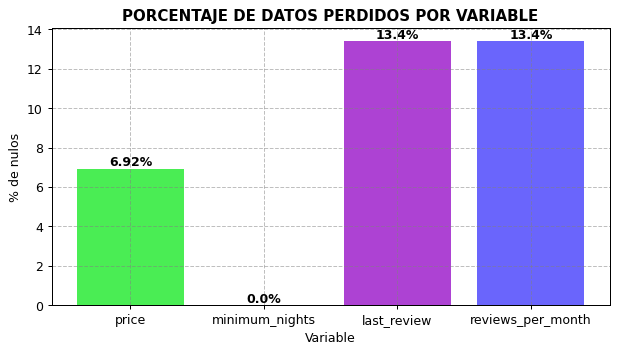
\includegraphics[width=0.78\textwidth]{01_datos_perdidos.png}
  \caption{Porcentaje de datos perdidos por variable tras eliminar columnas vacías.}
  \label{fig:datos_perdidos}
\end{figure}

Siguiendo la teoría de datos incompletos de \citet{little2019statistical}, se investigó el mecanismo detrás de cada patrón de ausencia antes de imputar o eliminar registros:

\begin{itemize}[leftmargin=1.5em]
  \item \textbf{Variable objetivo \texttt{price} (2,108 nulos; 6.92\%):} Al cruzar la ausencia de precio con \texttt{availability\_365}, se descubrió que \textbf{1,570 de los 2,108 anuncios sin precio (74.48\%)} tienen \texttt{availability\_365 = 0}, frente a solo \textbf{4 de los 28,360 anuncios con precio (0.01\%)}. Esto demuestra que los registros sin precio corresponden mayoritariamente a \textbf{anuncios inactivos o no publicados}. Imputar la variable respuesta con medias o medianas generaría observaciones artificiales y reduciría artificialmente la varianza; por ello, se \textbf{eliminaron} los 2,108 registros ($30{,}468 \rightarrow 28{,}360$). Además, la distribución de \texttt{room\_type} en los registros eliminados (65.13\% completos, 33.82\% privados, 1.00\% compartidos, 0.05\% hotel) resultó muy cercana a la del total, descartando un sesgo estructural por tipo de alojamiento.
  \item \textbf{Nulos estructurales en \texttt{last\_review} y \texttt{reviews\_per\_month} (4,083 en original; 3,582 tras filtrar \texttt{price}):} El cruce con \texttt{number\_of\_reviews} confirmó que en el \textbf{100\% de los casos} los anuncios con \texttt{last\_review} o \texttt{reviews\_per\_month} nulos tienen exactamente \texttt{number\_of\_reviews = 0} (0 casos con reseñas positivas y dato faltante). Se trata, por tanto, de \textbf{nulos estructurales} (el dato no falta por error, sino porque el alojamiento nunca ha recibido una reseña). En consecuencia: (i) se imputó \texttt{reviews\_per\_month = 0}; (ii) se creó la variable binaria \texttt{tiene\_resenas} ($1$ si \texttt{number\_of\_reviews > 0}, $0$ en caso contrario); y (iii) \texttt{last\_review} se convirtió al tipo \texttt{datetime} manteniendo su valor nulo estructural en la base legible, para transformarse posteriormente en días transcurridos (Paso~6).
  \item \textbf{Nulo puntual en \texttt{minimum\_nights} (1 registro):} Dado que esta variable presenta fuerte asimetría positiva, se imputó mediante la \textbf{mediana (1 noche)}, estimador robusto ante colas largas.
\end{itemize}

Para verificar que la eliminación de los 2,108 registros sin precio no distorsiona la distribución de las demás variables, la Tabla~\ref{tab:comp_nulos} compara los estadísticos descriptivos antes (\texttt{dataSet}) y después del filtrado (\texttt{filter\_data}).

\begin{table}[htbp]
\centering
\caption{Comparación de estadísticos descriptivos antes (\texttt{dataSet}) y después de eliminar nulos en \texttt{price} (\texttt{filter\_data}).}
\label{tab:comp_nulos}
\scriptsize
\renewcommand{\arraystretch}{1.15}
\begin{tabular}{l r r r r r r}
\toprule
\rowcolor{TableHeader}
\textbf{Variable (Etapa)} & \textbf{Conteo} & \textbf{Media} & \textbf{Desv. Est.} & \textbf{Q1 (25\%)} & \textbf{Mediana} & \textbf{Q3 (75\%)} \\
\midrule
\texttt{minimum\_nights} (Original) & 30,467 & 2.92 & 16.03 & 1.00 & 1.00 & 2.00 \\
\texttt{minimum\_nights} (Filtrada) & 28,359 & 2.33 &  9.92 & 1.00 & 1.00 & 2.00 \\
\midrule
\texttt{number\_of\_reviews} (Original) & 30,468 & 58.92 & 95.34 & 4.00 & 22.00 & 75.00 \\
\texttt{number\_of\_reviews} (Filtrada) & 28,360 & 60.70 & 96.67 & 4.00 & 23.00 & 78.00 \\
\midrule
\texttt{reviews\_per\_month} (Original) & 26,385 & 2.01 & 2.28 & 0.57 & 1.47 & 2.79 \\
\texttt{reviews\_per\_month} (Filtrada) & 24,778 & 2.07 & 2.30 & 0.63 & 1.56 & 2.86 \\
\midrule
\texttt{availability\_365} (Original) & 30,468 & 247.83 & 119.10 & 163.00 & 296.00 & 349.00 \\
\texttt{availability\_365} (Filtrada) & 28,360 & 262.06 & 106.03 & 188.00 & 306.00 & 350.00 \\
\bottomrule
\end{tabular}
\end{table}

Como se aprecia en la Tabla~\ref{tab:comp_nulos}, los cuartiles y medianas permanecen estables (por ejemplo, \texttt{minimum\_nights} conserva exactamente Q1=1, mediana=1 y Q3=2; \texttt{number\_of\_reviews} pasa de mediana 22 a 23), mientras que \texttt{availability\_365} aumenta coherentemente al remover los anuncios inactivos con disponibilidad cero.

\subsection{Paso 3: Detección y corrección de inconsistencias}
\label{subsec:paso3}

Sobre los 28,360 registros activos se ejecutó una auditoría sistemática compuesta por \textbf{13 reglas de consistencia} (duplicidad exacta y clonación, integridad de llaves, rangos numéricos y geográficos, consistencia temporal, coherencia lógica entre columnas y formato de cadenas de texto). La fecha de corte detectada a partir de la última reseña fue el \textbf{25 de septiembre de 2026}. Los resultados se detallan en la Tabla~\ref{tab:reglas_inconsistencias}.

\begin{table}[htbp]
\centering
\caption{Resultados de la auditoría de 13 reglas de consistencia ($n = 28{,}360$).}
\label{tab:reglas_inconsistencias}
\footnotesize
\renewcommand{\arraystretch}{1.15}
\begin{tabularx}{\textwidth}{Y r c}
\toprule
\rowcolor{TableHeader}
\textbf{Regla de consistencia verificada} & \textbf{Registros con fallo} & \textbf{Estado inicial} \\
\midrule
Registros duplicados considerando todas las columnas & 0 & Correcto \\
\rowcolor{WarnBg}
\textbf{Duplicados ignorando \texttt{id} (mismo anuncio repetido/clonado)} & \textbf{79} & \textbf{Corregido} \\
Identificador \texttt{id} repetido & 0 & Correcto \\
Precio no positivo (\texttt{price <= 0}) & 0 & Correcto \\
Noches mínimas menores a 1 (\texttt{minimum\_nights < 1}) & 0 & Correcto \\
Noches mínimas mayores a 1 año (\texttt{minimum\_nights > 365}) & 0 & Correcto \\
Disponibilidad fuera de rango (\texttt{availability\_365} $\notin [0, 365]$) & 0 & Correcto \\
Reseñas del último año mayores al total (\texttt{reviews\_ltm > reviews}) & 0 & Correcto \\
Anuncios con 0 reseñas pero fecha de última reseña registrada & 0 & Correcto \\
Latitud fuera de límites geográficos de CDMX ($[19.0,\; 19.6]$) & 0 & Correcto \\
Longitud fuera de límites geográficos de CDMX ($[-99.4,\; -98.9]$) & 0 & Correcto \\
Fecha de última reseña posterior a la fecha de corte (2026-09-25) & 0 & Correcto \\
Espacios sobrantes en texto (\texttt{neighbourhood} o \texttt{room\_type}) & 0 & Correcto \\
\bottomrule
\end{tabularx}
\end{table}

La única inconsistencia real identificada fue la existencia de \textbf{79 anuncios clonados}: registros que comparten exactamente el mismo anfitrión, alcaldía, coordenadas geográficas, tipo de alojamiento, precio, condiciones de reserva y reseñas, diferenciándose únicamente en el identificador \texttt{id}. A modo de evidencia, la Tabla~\ref{tab:ejemplo_duplicados} muestra un extracto de anuncios clonados pertenecientes al anfitrión \texttt{487725046}.

\begin{table}[htbp]
\centering
\caption{Ejemplo de anuncios duplicados con distinto \texttt{id} detectados en la auditoría.}
\label{tab:ejemplo_duplicados}
\scriptsize
\renewcommand{\arraystretch}{1.15}
\begin{tabular}{r r l l r r r}
\toprule
\rowcolor{TableHeader}
\textbf{\texttt{id}} & \textbf{\texttt{host\_id}} & \textbf{\texttt{neighbourhood}} & \textbf{\texttt{room\_type}} & \textbf{\texttt{price}} & \textbf{\texttt{latitude}} & \textbf{\texttt{longitude}} \\
\midrule
1442212003884952561 & 487725046 & Cuauhtémoc & Private room & 1,630.0 & 19.405605 & $-99.170359$ \\
1442229920632599146 & 487725046 & Cuauhtémoc & Private room & 1,630.0 & 19.405605 & $-99.170359$ \\
\rowcolor{RowStripe}
1442965869663446178 & 487725046 & Cuauhtémoc & Private room & 1,730.0 & 19.405605 & $-99.170359$ \\
\rowcolor{RowStripe}
1442985817530903287 & 487725046 & Cuauhtémoc & Private room & 1,730.0 & 19.405605 & $-99.170359$ \\
\rowcolor{RowStripe}
1442989718286270875 & 487725046 & Cuauhtémoc & Private room & 1,730.0 & 19.405605 & $-99.170359$ \\
\bottomrule
\end{tabular}
\end{table}

\textbf{Correcciones aplicadas:} (1) se eliminaron los 79 anuncios duplicados conservando la primera aparición (\texttt{keep="first"}), pasando de 28,360 a \textbf{28,281 registros}; (2) se aplicó \texttt{str.strip()} preventivo sobre \texttt{neighbourhood} y \texttt{room\_type}, confirmando la ortografía uniforme de las 16 alcaldías y los 4 tipos de alojamiento; y (3) como regla de negocio preventiva, se acotó \texttt{minimum\_nights} a un tope máximo de 365 noches y se convirtió a tipo entero (\texttt{int64}).

\subsection{Paso 4: Tratamiento de variables numéricas y valores atípicos}
\label{subsec:paso4}

Se calculó un perfil estadístico completo para las siete variables numéricas principales ---incluyendo media, mediana, cuartiles, rango intercuartílico ($\text{RIC} = Q_3 - Q_1$), límite superior de Tukey ($Q_3 + 1.5\cdot\text{RIC}$), coeficiente de asimetría y número de atípicos bajo la regla estándar \citep{tukey1977exploratory}--- resumido en la Tabla~\ref{tab:perfil_numericas}.

\begin{table}[htbp]
\centering
\caption{Diagnóstico descriptivo y detección de atípicos (RIC) en variables numéricas ($n = 28{,}281$).}
\label{tab:perfil_numericas}
\scriptsize
\setlength{\tabcolsep}{4pt}
\renewcommand{\arraystretch}{1.15}
\begin{tabular}{l r r r r r r r r r}
\toprule
\rowcolor{TableHeader}
\textbf{Variable} & \textbf{Media} & \textbf{Mediana} & \textbf{Mín.} & \textbf{Q1} & \textbf{Q3} & \textbf{Máx.} & \textbf{RIC} & \textbf{Asim.} & \textbf{Atíp.} \\
\midrule
\texttt{price}                         & 2,341.51 & 1,500.00 & 137.0 & 941.00 & 2,328.00 & 1,826,199 & 1,387.00 &  96.87 & 2,099 \\
\rowcolor{RowStripe}
\texttt{minimum\_nights}               &     2.34 &     1.00 &   1.0 &   1.00 &     2.00 &       365 &     1.00 &  27.63 & 1,851 \\
\texttt{number\_of\_reviews}           &    60.87 &    23.00 &   0.0 &   4.00 &    79.00 &     1,893 &    75.00 &   3.78 & 2,223 \\
\rowcolor{RowStripe}
\texttt{reviews\_per\_month}           &     1.81 &     1.25 &   0.0 &   0.31 &     2.64 &    107.56 &     2.33 &   7.79 &   959 \\
\texttt{calculated\_host\_listings}    &    14.67 &     4.00 &   1.0 &   1.00 &    12.00 &       187 &    11.00 &   3.69 & 3,568 \\
\rowcolor{RowStripe}
\texttt{availability\_365}             &   262.06 &   306.00 &   0.0 & 188.00 &   350.00 &       365 &   162.00 & $-0.92$ &    0 \\
\texttt{number\_of\_reviews\_ltm}      &    17.34 &    10.00 &   0.0 &   1.00 &    26.00 &     1,241 &    25.00 &   9.27 & 1,027 \\
\bottomrule
\end{tabular}
\end{table}

El diagnóstico evidencia que \texttt{price} presenta una \textbf{asimetría positiva extrema (96.87)}, ocasionada por precios irreales que alcanzan \$1,826,199 MXN por noche (por ejemplo, una habitación privada en Cuauhtémoc listada en \$1.83 millones y otra en Tlalpan en \$1.00 millón; ver Tabla~\ref{tab:precios_extremos}), los cuales suelen reflejar errores de captura o tarifas simbólicas usadas por anfitriones para bloquear fechas.

\begin{table}[htbp]
\centering
\caption{Ejemplos de los precios más extremos detectados antes de la depuración.}
\label{tab:precios_extremos}
\scriptsize
\renewcommand{\arraystretch}{1.15}
\begin{tabular}{r l l r r}
\toprule
\rowcolor{TableHeader}
\textbf{\texttt{id}} & \textbf{\texttt{neighbourhood}} & \textbf{\texttt{room\_type}} & \textbf{\texttt{price} (MXN)} & \textbf{\texttt{number\_of\_reviews}} \\
\midrule
38778769            & Cuauhtémoc     & Private room    & 1,826,199.0 & 227 \\
892676742760732948  & Tlalpan        & Private room    & 1,000,300.0 &   3 \\
1603720147099182676 & Miguel Hidalgo & Entire home/apt &   790,057.0 &   0 \\
812373795418706059  & Cuauhtémoc     & Entire home/apt &   500,000.0 &   6 \\
666513486864947875  & Miguel Hidalgo & Entire home/apt &   152,220.0 &   0 \\
901962391238044233  & Tlalpan        & Entire home/apt &   141,000.0 &   0 \\
\bottomrule
\end{tabular}
\end{table}

\textbf{Criterio para \texttt{price}:} Aplicar el criterio de Tukey directamente sobre la escala original fija un límite superior de \$4,408.50 MXN, lo que eliminaría 2,099 registros (7.42\%), descartando numerosos alojamientos reales de segmento residencial alto o lujo (e.g., casas completas en Polanco, Condesa o Santa Fe). En contraste, la transformación logarítmica $Y = \ln(\texttt{price})$ exhibe una distribución aproximadamente simétrica y acampanada (Figura~\ref{fig:price_log}). Por ello, se aplicó la regla de Tukey sobre $\ln(\texttt{price})$:
\begin{align*}
L_{\inf} &= \exp\!\left(Q_{1,\ln} - 1.5\cdot \text{RIC}_{\ln}\right) = \$241.82\text{ MXN}, \\
L_{\sup} &= \exp\!\left(Q_{3,\ln} + 1.5\cdot \text{RIC}_{\ln}\right) = \$9{,}058.85\text{ MXN}.
\end{align*}

Bajo este criterio se identificaron y eliminaron \textbf{698 anuncios atípicos (2.47\% de los 28,281 registros)}: 145 por debajo de \$241.82 y 553 por encima de \$9,058.85, quedando \textbf{27,583 registros finales}.

\begin{figure}[htbp]
  \centering
  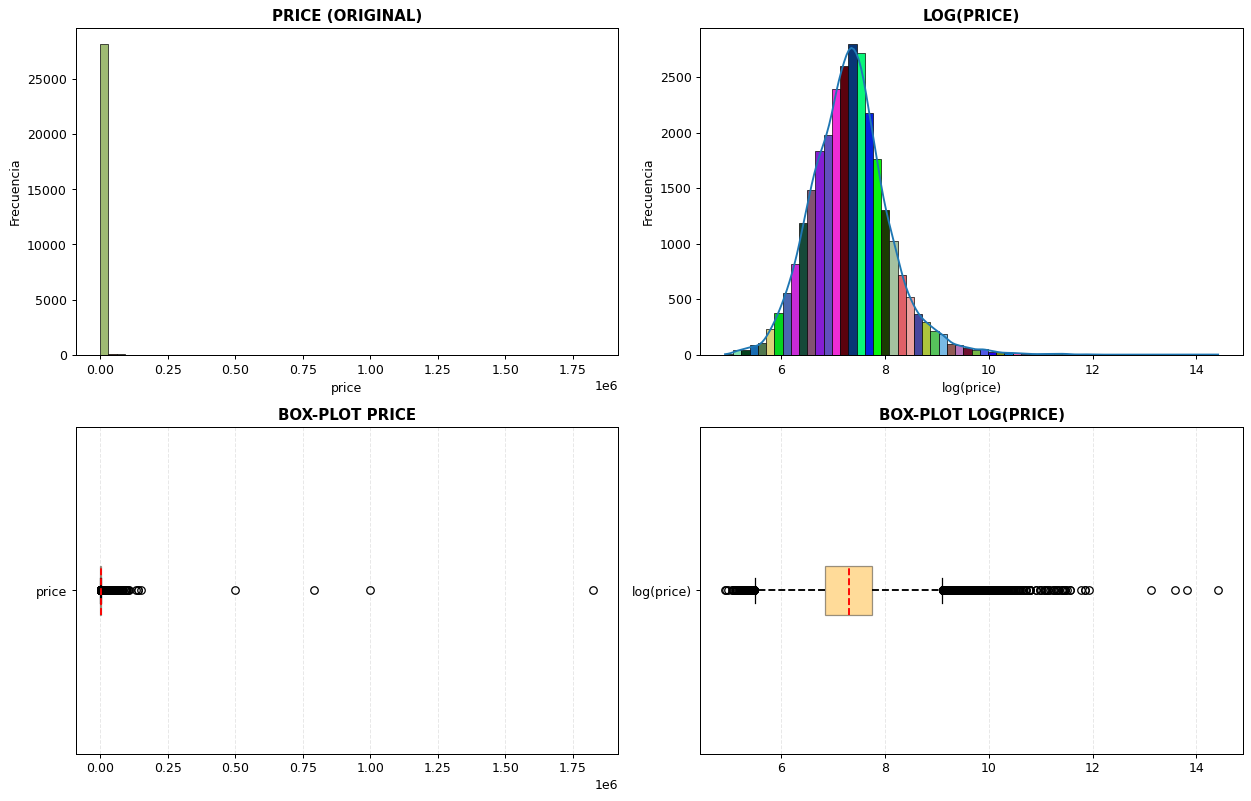
\includegraphics[width=0.92\textwidth]{02_price_original_vs_log.png}
  \caption{Comparación de histogramas y diagramas de caja de \texttt{price} en escala original vs.\ $\ln(\texttt{price})$.}
  \label{fig:price_log}
\end{figure}

La Figura~\ref{fig:price_antes_despues} y la Tabla~\ref{tab:price_antes_despues} demuestran la eficacia del criterio: la desviación estándar cae de \$14,113.71 a \$1,366.90 MXN y la asimetría se reduce de 96.87 a \textbf{2.09} (y a apenas \textbf{0.09} en \texttt{log\_price}), mientras que la mediana (\$1,500 $\rightarrow$ \$1,490) y el rango intercuartílico permanecen prácticamente inalterados.

\begin{figure}[htbp]
  \centering
  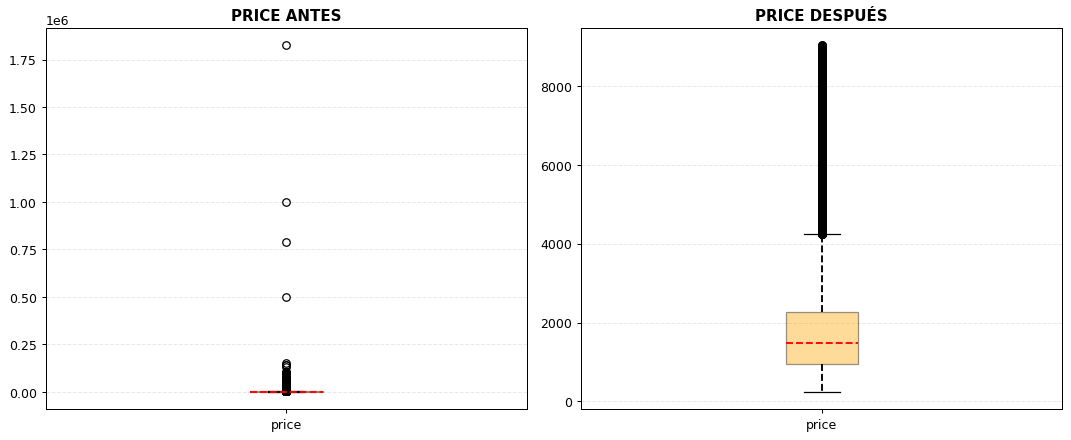
\includegraphics[width=0.84\textwidth]{03_price_antes_despues.png}
  \caption{Diagrama de caja de \texttt{price} antes y después de la depuración de atípicos con Tukey sobre $\ln(\texttt{price})$.}
  \label{fig:price_antes_despues}
\end{figure}

\begin{table}[htbp]
\centering
\caption{Efecto del tratamiento de valores atípicos sobre los estadísticos de \texttt{price}.}
\label{tab:price_antes_despues}
\footnotesize
\renewcommand{\arraystretch}{1.15}
\begin{tabular}{l r r}
\toprule
\rowcolor{TableHeader}
\textbf{Estadístico} & \textbf{Antes ($n = 28{,}281$)} & \textbf{Después ($n = 27{,}583$)} \\
\midrule
Media (MXN)               &     2,341.51 & 1,845.83 \\
Desviación estándar (MXN) &    14,113.71 & 1,366.90 \\
Mínimo (MXN)              &       137.00 &   243.00 \\
Q1 -- 25\% (MXN)          &       941.00 &   940.00 \\
Mediana -- 50\% (MXN)     &     1,500.00 & 1,490.00 \\
Q3 -- 75\% (MXN)          &     2,328.00 & 2,260.00 \\
Máximo (MXN)              & 1,826,199.00 & 9,034.00 \\
Asimetría (\textit{skewness}) &    96.87 &     2.09 \\
\bottomrule
\end{tabular}
\end{table}

\textbf{Criterio para el resto de variables numéricas:} Aunque \texttt{minimum\ub nights}, \texttt{number\ub of\ub reviews}, \texttt{reviews\ub per\ub month}, \texttt{calculated\ub host\ub listings\ub count} y \texttt{number\ub of\ub reviews\ub ltm} presentan colas largas a la derecha, sus valores altos representan \textbf{fenómenos legítimos del negocio} (alquileres de mediana/larga estancia, alojamientos históricos altamente populares y operadores profesionales con múltiples propiedades). Eliminarlos mutilaría información real del mercado, por lo que \textbf{se conservaron íntegros} y se prescribe emplear estadísticos robustos (mediana, RIC, correlación de Spearman) en las etapas analíticas. Por su parte, \texttt{availability\ub 365} está naturalmente acotada en $[0, 365]$ y no presenta valores atípicos.

\subsection{Paso 5: Tratamiento de variables categóricas}
\label{subsec:paso5}

Se examinaron las frecuencias absolutas, proporciones y estadísticos de precio para las dos variables categóricas originales (\texttt{room\_type} y \texttt{neighbourhood}) sobre los 27,583 registros depurados. Las Tablas~\ref{tab:cat_room_type} y~\ref{tab:cat_neighbourhood} presentan estos resultados.

\begin{table}[htbp]
\centering
\caption{Distribución de frecuencias y precio (MXN) por tipo de alojamiento (\texttt{room\_type}).}
\label{tab:cat_room_type}
\footnotesize
\renewcommand{\arraystretch}{1.15}
\begin{tabular}{l r r r r}
\toprule
\rowcolor{TableHeader}
\textbf{Tipo de alojamiento} & \textbf{Frec.\ ($N$)} & \textbf{Part.\ (\%)} & \textbf{Mediana (MXN)} & \textbf{Media (MXN)} \\
\midrule
\texttt{Entire home/apt} & 18,463 & 66.94 & 1,800.00 & 2,190.75 \\
\texttt{Hotel room}      &     62 &  0.22 & 1,724.00 & 2,890.81 \\
\texttt{Private room}    &  8,856 & 32.11 &   849.00 & 1,144.63 \\
\texttt{Shared room}     &    202 &  0.73 &   445.50 &   741.48 \\
\midrule
\textbf{Total}           & \textbf{27,583} & \textbf{100.00} & \textbf{1,490.00} & \textbf{1,845.83} \\
\bottomrule
\end{tabular}
\end{table}

\begin{table}[htbp]
\centering
\caption{Distribución de frecuencias y precio (MXN) por alcaldía (\texttt{neighbourhood}), ordenada por precio mediano descendente.}
\label{tab:cat_neighbourhood}
\scriptsize
\renewcommand{\arraystretch}{1.12}
\begin{tabular}{l r r r r}
\toprule
\rowcolor{TableHeader}
\textbf{Alcaldía (\texttt{neighbourhood})} & \textbf{Frecuencia ($N$)} & \textbf{Participación (\%)} & \textbf{Precio Mediano} & \textbf{Precio Medio} \\
\midrule
Miguel Hidalgo          &  4,275 & 15.50 & 1,850.00 & 2,287.83 \\
Cuajimalpa de Morelos   &    354 &  1.28 & 1,789.00 & 2,020.81 \\
Cuauhtémoc              & 12,820 & 46.48 & 1,673.00 & 2,020.82 \\
Álvaro Obregón          &    898 &  3.26 & 1,324.00 & 1,598.57 \\
Benito Juárez           &  3,166 & 11.48 & 1,200.00 & 1,479.19 \\
Coyoacán                &  2,001 &  7.25 & 1,190.00 & 1,548.42 \\
Iztacalco               &    553 &  2.00 & 1,160.00 & 1,328.89 \\
Xochimilco              &    172 &  0.62 & 1,044.50 & 1,548.30 \\
La Magdalena Contreras  &    116 &  0.42 & 1,019.50 & 1,568.72 \\
Tlalpan                 &    882 &  3.20 & 1,000.00 & 1,594.41 \\
Venustiano Carranza     &  1,005 &  3.64 &   999.00 & 1,242.09 \\
Azcapotzalco            &    385 &  1.40 &   921.00 & 1,169.70 \\
Gustavo A.\ Madero      &    541 &  1.96 &   838.00 & 1,062.69 \\
Iztapalapa              &    349 &  1.27 &   827.00 & 1,054.74 \\
Milpa Alta              &     24 &  0.09 &   814.00 & 1,253.00 \\
Tláhuac                 &     42 &  0.15 &   679.50 &   778.29 \\
\midrule
\textbf{Total}          & \textbf{27,583} & \textbf{100.00} & \textbf{1,490.00} & \textbf{1,845.83} \\
\bottomrule
\end{tabular}
\end{table}

\textbf{Criterio sobre categorías minoritarias:} Las clases con menor volumen de observaciones ---\texttt{Shared room} (202; 0.73\%), \texttt{Hotel room} (62; 0.22\%), Milpa Alta (24; 0.09\%) y Tláhuac (42; 0.15\%)--- \textbf{se conservaron sin reagrupar} porque constituyen segmentos reales y bien definidos del mercado de la Ciudad de México. No obstante, cualquier inferencia sobre estos grupos deberá interpretarse con cautela por su reducido tamaño de muestra.

\subsection{Paso 6: Transformación de datos y codificación}
\label{subsec:paso6}

Para habilitar el uso de técnicas estadísticas paramétricas, no paramétricas y modelos de aprendizaje automático, se aplicaron cinco transformaciones documentadas en la Tabla~\ref{tab:transformaciones}:

\begin{table}[htbp]
\centering
\caption{Resumen de variables derivadas y esquema de codificación aplicados (Paso 6).}
\label{tab:transformaciones}
\footnotesize
\renewcommand{\arraystretch}{1.2}
\begin{tabularx}{\textwidth}{>{\raggedright\arraybackslash}p{2.7cm} >{\raggedright\arraybackslash}p{4.3cm} Y}
\toprule
\rowcolor{TableHeader}
\textbf{Transformación} & \textbf{Variable(s) nueva(s)} & \textbf{Criterio y justificación} \\
\midrule
Logaritmo natural & \texttt{log\_price} & Corrige la asimetría del precio ($\text{media}=7.30$, $\text{DE}=0.66$, $\text{mín}=5.49$, $\text{máx}=9.11$, asimetría $\approx 0.09$), acercándola a la normalidad. \\
\rowcolor{RowStripe}
Fecha a días desde corte & \texttt{dias\ub desde\ub ultima\ub resena} & Transforma \texttt{last\_review} en antigüedad numérica respecto al 25/09/2026 (mediana: 35 días). A los 3,254 anuncios sin reseña se les asigna el máximo observado (4,250 días) en conjunto con \texttt{tiene\_resenas = 0}. \\
Indicador binario & \texttt{tiene\_resenas} & Preserva explícitamente la información del nulo estructural (24,329 anuncios con reseñas [88.20\%] vs.\ 3,254 sin reseñas [11.80\%]). \\
\rowcolor{RowStripe}
Discretización & \texttt{tipo\_estancia} & Agrupa \texttt{minimum\_nights} en segmentos de negocio: Corta 1--7 noches (26,999; 97.88\%), Media 8--29 noches (374; 1.36\%) y Larga 30+ noches (210; 0.76\%). \\
\textit{One-hot encoding} & \texttt{room\_*}, \texttt{alc\_*}, \texttt{estancia\_*} & Codifica variables nominales en columnas binarias 0/1 (\texttt{dtype=int}) para evitar imponer un orden numérico artificial inexistente \citep{garcia2015data}. \\
\bottomrule
\end{tabularx}
\end{table}

Como resultado, se generaron dos versiones sincronizadas de la base de datos: la versión legible \texttt{df} (\textbf{27,583 $\times$ 18}) y la versión completamente numérica \texttt{df\_cod} (\textbf{27,583 $\times$ 37}, detallada en el Anexo~\ref{anexo:columnas}), en la cual se excluye la fecha cruda \texttt{last\_review} al quedar representada sin pérdida de información por \texttt{dias\_desde\_ultima\_resena} y \texttt{tiene\_resenas}.

% ------------------------------------------------------------------------------
\section{Interpretación de los análisis exploratorios gráficos}
\label{sec:eda_graficos}

A continuación se interpretan las visualizaciones construidas durante el análisis exploratorio sobre la base depurada, orientadas a parametrizar las variables y evaluar de forma preliminar la hipótesis de trabajo.

\subsection{Frecuencias y precios medianos de variables categóricas}

Las Figuras~\ref{fig:frec_cat} y~\ref{fig:mediana_cat} revelan una marcada concentración geográfica y una fuerte diferenciación tarifaria por categoría.

\begin{figure}[htbp]
  \centering
  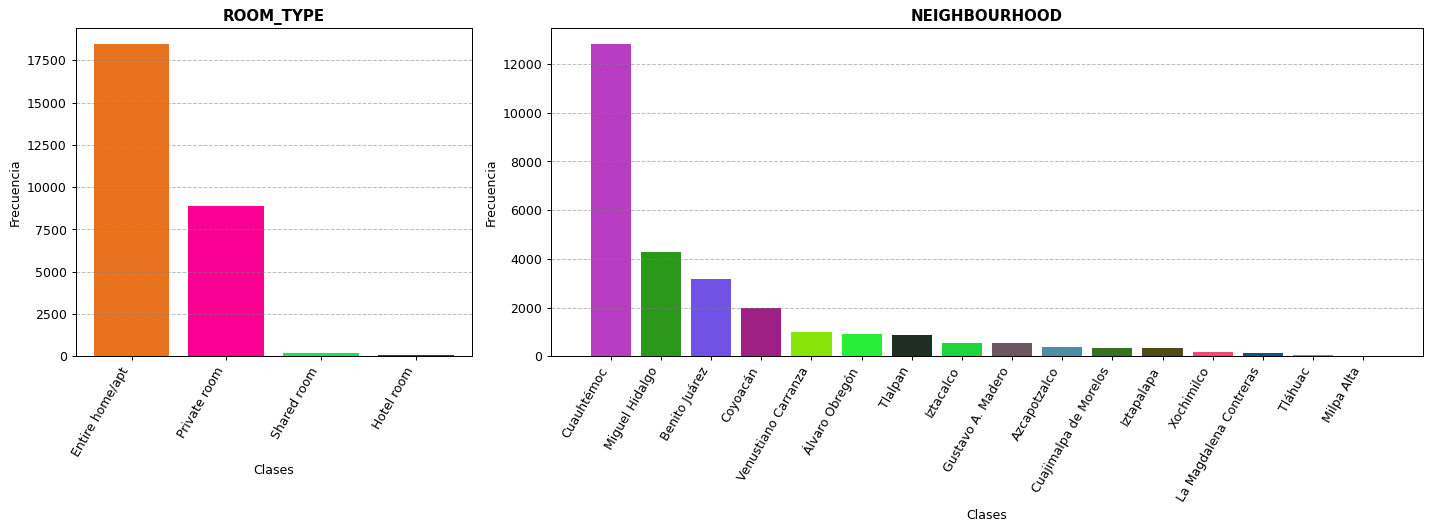
\includegraphics[width=\textwidth]{04_frecuencias_categoricas.png}
  \caption{Distribución de frecuencias de \texttt{room\_type} y \texttt{neighbourhood} en la base depurada.}
  \label{fig:frec_cat}
\end{figure}

\begin{figure}[htbp]
  \centering
  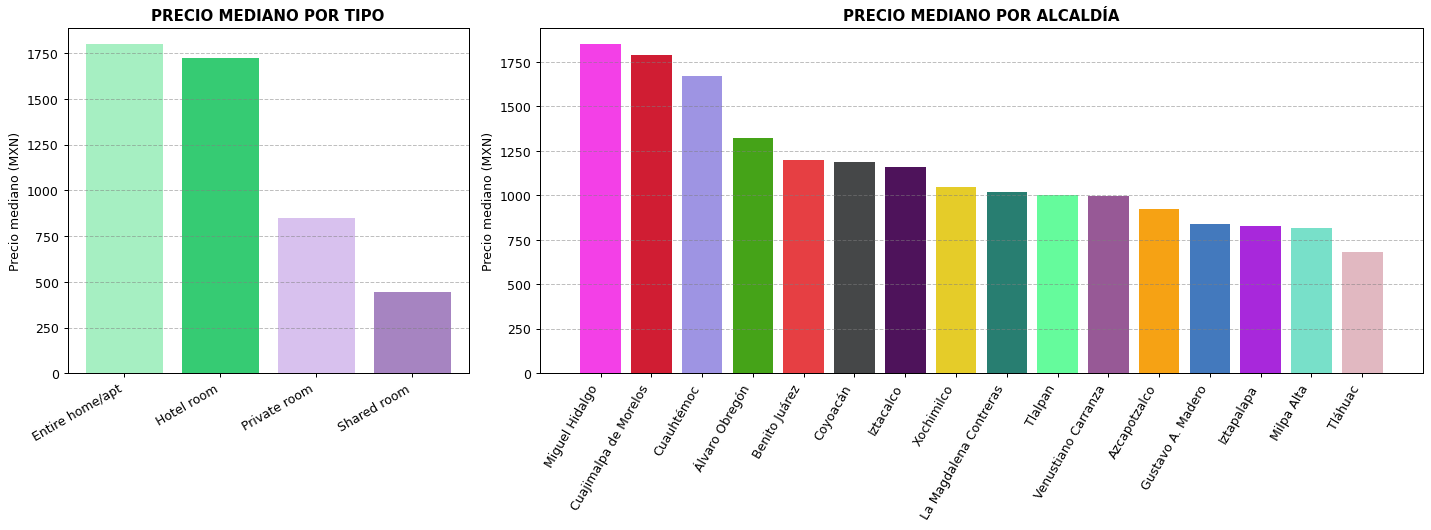
\includegraphics[width=\textwidth]{05_precio_mediano_tipo_alcaldia.png}
  \caption{Precio mediano por noche (MXN) según tipo de alojamiento y alcaldía.}
  \label{fig:mediana_cat}
\end{figure}

\begin{itemize}[leftmargin=1.5em]
  \item \textbf{Dominio del alojamiento completo:} \texttt{Entire home/apt} representa el \textbf{66.94\%} de la oferta (18,463 anuncios) y \texttt{Private room} el \textbf{32.11\%} (8,856), sumando en conjunto el 99.05\% del mercado. El precio mediano de un alojamiento completo (\$1,800 MXN) equivale a \textbf{2.12 veces} el de una habitación privada (\$849 MXN) y a \textbf{4.04 veces} el de una habitación compartida (\$445.50 MXN).
  \item \textbf{Alta concentración territorial:} La alcaldía Cuauhtémoc concentra por sí sola el \textbf{46.48\%} de los anuncios (12,820); al sumar Miguel Hidalgo (15.50\%) y Benito Juárez (11.48\%), apenas tres alcaldías aglutinan el \textbf{73.46\%} de toda la oferta capitalina.
  \item \textbf{Brecha territorial de precios:} Los precios medianos más altos corresponden a Miguel Hidalgo (\$1,850 MXN), Cuajimalpa de Morelos (\$1,789 MXN) y Cuauhtémoc (\$1,673 MXN), casi triplicando la mediana observada en alcaldías periféricas como Tláhuac (\$679.50 MXN), Milpa Alta (\$814 MXN) e Iztapalapa (\$827 MXN).
\end{itemize}

\subsection{Distribuciones univariadas de las variables numéricas}

La Figura~\ref{fig:hist_num} muestra los histogramas con estimación de densidad kernel (KDE) de seis variables numéricas clave tras la depuración.

\begin{figure}[htbp]
  \centering
  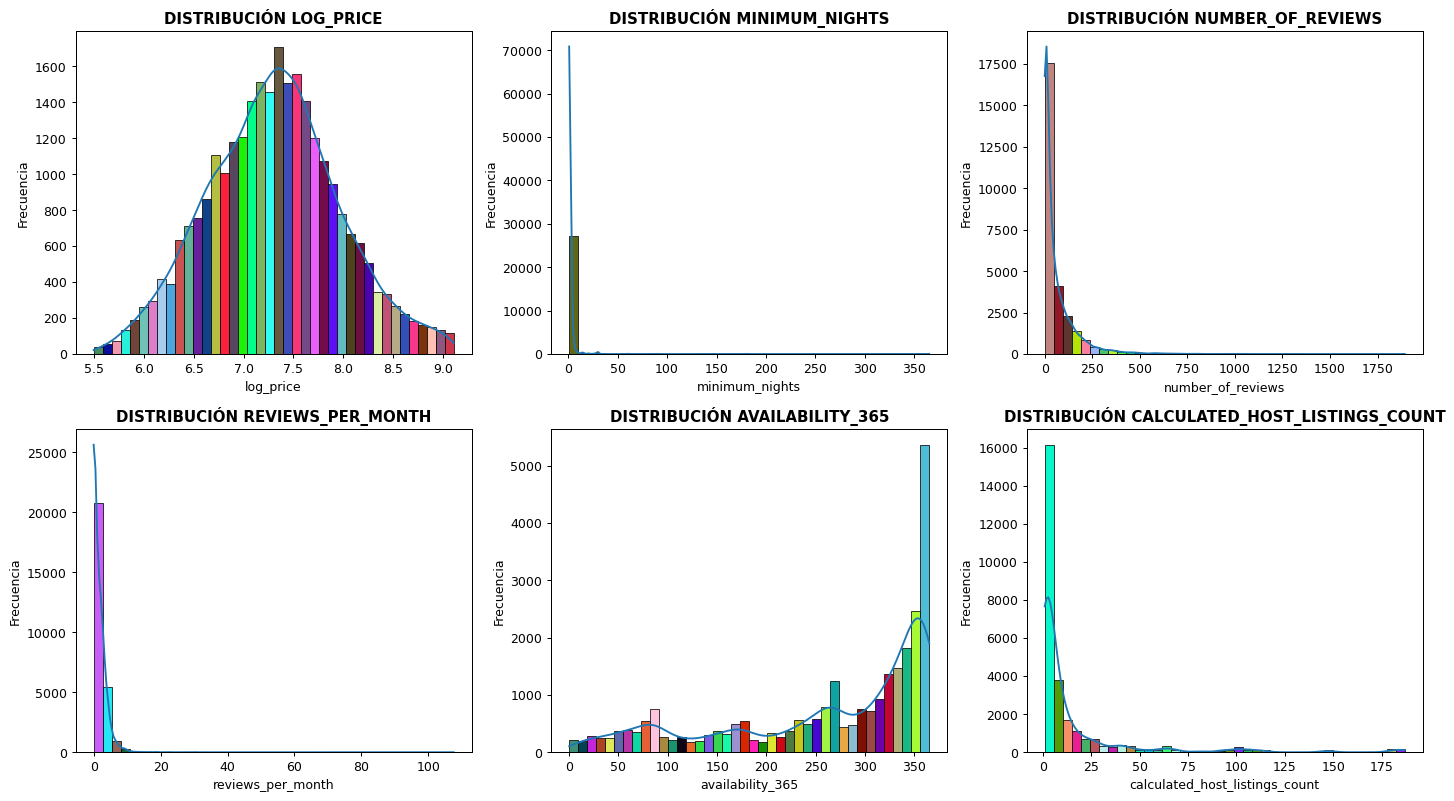
\includegraphics[width=\textwidth]{06_histogramas_numericas.png}
  \caption{Histogramas y curvas de densidad de las principales variables numéricas en la base depurada.}
  \label{fig:hist_num}
\end{figure}

Se observan tres patrones distribucionales bien diferenciados: (1) \texttt{log\_price} presenta una forma acampanada casi simétrica centrada en $7.30$ ($\approx \$1{,}480$ MXN), validando su idoneidad como variable dependiente para futuros modelos lineales; (2) \texttt{minimum\_nights}, \texttt{number\_of\_reviews}, \texttt{reviews\_per\_month} y \texttt{calculated\_host\_listings\_count} muestran una asimetría positiva pronunciada, donde la mayoría de los anuncios opera con valores bajos y una minoría concentra volúmenes muy elevados; y (3) \texttt{availability\_365} presenta asimetría negativa (mediana de 306 días), reflejando que la mayoría de los anuncios mantiene disponibilidad casi permanente durante el año.

\subsection{Matriz de correlación de Spearman}

Dada la no normalidad y las colas largas de varias variables numéricas, se empleó el coeficiente de correlación por rangos de Spearman ($\rho$) \citep{spearman1904proof}, el cual es robusto ante valores extremos y capta relaciones monótonas (Figura~\ref{fig:matriz_corr}).

\begin{figure}[htbp]
  \centering
  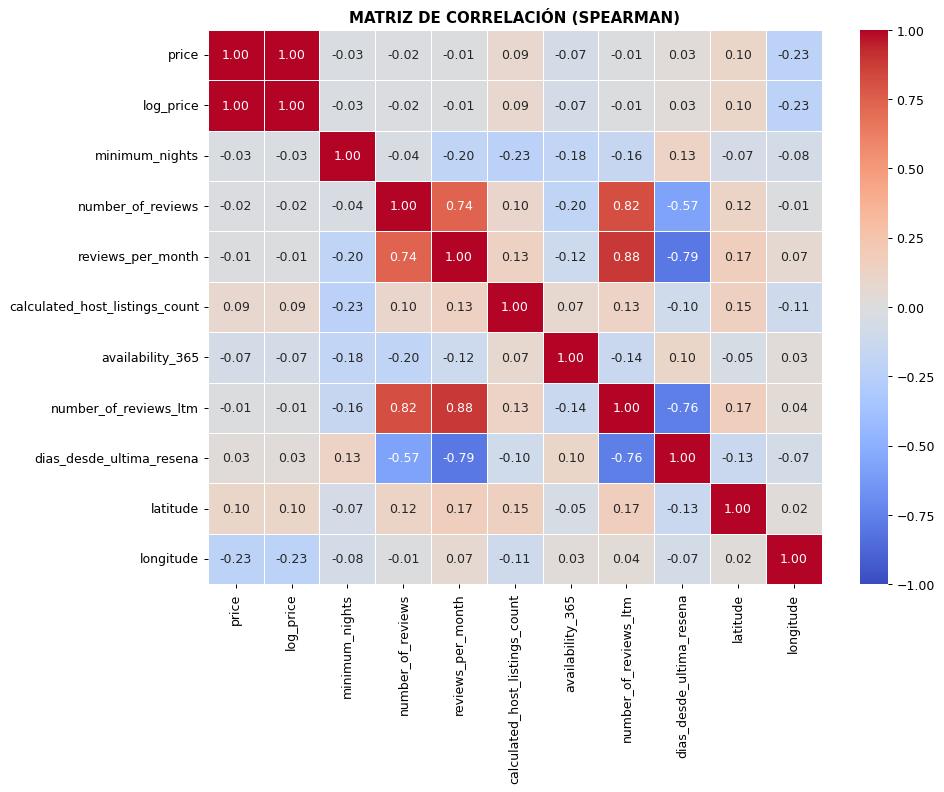
\includegraphics[width=0.86\textwidth]{07_matriz_correlacion.png}
  \caption{Matriz de correlación de Spearman ($\rho$) entre variables numéricas de la base depurada.}
  \label{fig:matriz_corr}
\end{figure}

El mapa de calor aporta dos hallazgos decisivos para el modelado posterior:
\begin{enumerate}[leftmargin=1.5em]
  \item \textbf{Correlaciones débiles entre variables numéricas y precio:} Ninguna variable numérica muestra una asociación lineal o monótona fuerte con \texttt{price}. Las de mayor magnitud son precisamente las coordenadas geográficas: \texttt{longitude} ($\rho = -0.226$, indicando que los precios aumentan hacia el poniente de la ciudad) y \texttt{latitude} ($\rho = 0.102$), seguidas de \texttt{calculated\_host\_listings\_count} ($\rho = 0.086$) y \texttt{availability\_365} ($\rho = -0.073$). Todas las variables de reseñas presentan correlaciones prácticamente nulas con el precio (\texttt{number\_of\_reviews}: $-0.018$; \texttt{reviews\_per\_month}: $-0.009$; \texttt{number\_of\_reviews\_ltm}: $-0.008$; \texttt{dias\_desde\_ultima\_resena}: $0.026$).
  \item \textbf{Fuerte multicolinealidad entre métricas de reseñas:} Las variables de actividad presentan correlaciones muy altas entre sí: \texttt{reviews\ub per\ub month} con \texttt{number\ub of\ub reviews\ub ltm} ($\rho = 0.88$), \texttt{number\ub of\ub reviews} con \texttt{number\ub of\ub reviews\ub ltm} ($\rho = 0.82$), \texttt{number\ub of\ub reviews} con \texttt{reviews\ub per\ub month} ($\rho = 0.74$) y \texttt{dias\ub desde\ub ultima\ub resena} de forma inversa con todas ellas ($\rho$ entre $-0.57$ y $-0.79$). Incluirlas simultáneamente en una regresión provocaría multicolinealidad severa.
\end{enumerate}

\subsection{Dispersión del precio por tipo de alojamiento y alcaldías principales}

La Figura~\ref{fig:boxplots_cat} complementa las medianas con la dispersión completa del precio por \texttt{room\_type} y en las ocho alcaldías con mayor número de anuncios.

\begin{figure}[htbp]
  \centering
  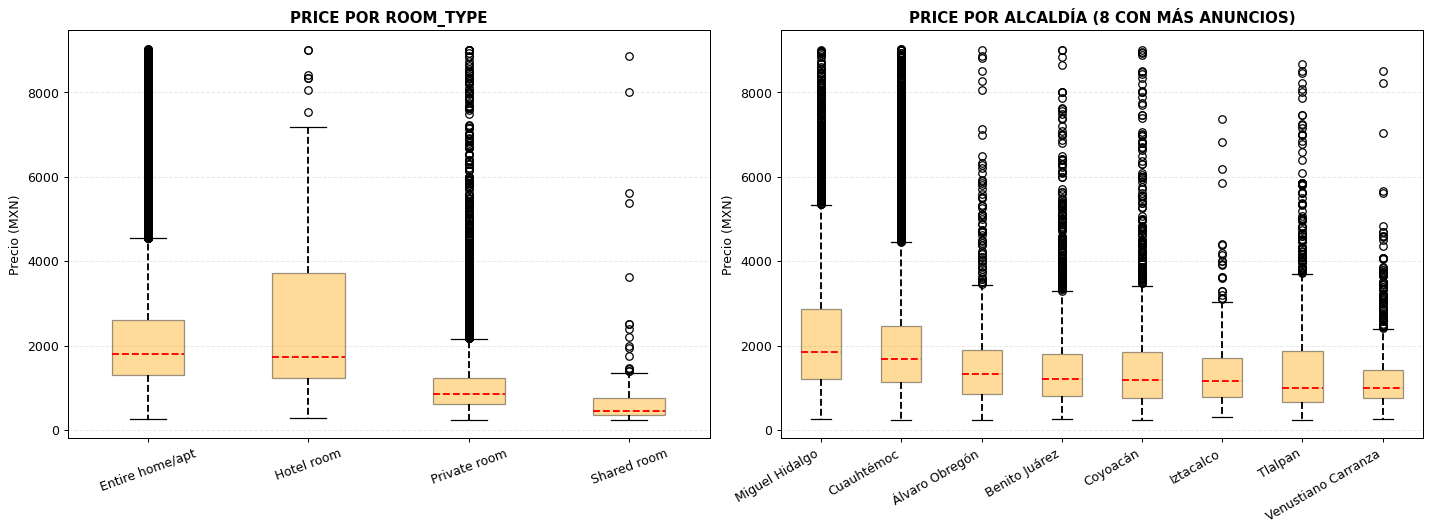
\includegraphics[width=\textwidth]{08_boxplot_precio_tipo_alcaldia.png}
  \caption{Diagramas de caja de \texttt{price} por tipo de alojamiento y por las 8 alcaldías con mayor oferta.}
  \label{fig:boxplots_cat}
\end{figure}

Las cajas confirman una separación clara entre los segmentos: el tercer cuartil de las habitaciones privadas y compartidas se ubica por debajo de la mediana de los alojamientos completos. Asimismo, aunque \texttt{Hotel room} tiene una mediana similar a \texttt{Entire home/apt} (\$1,724 vs.\ \$1,800 MXN), exhibe una caja considerablemente más amplia debido a la convivencia de hoteles económicos y boutiques de gama alta con un tamaño muestral reducido ($N=62$). Entre las ocho alcaldías con mayor volumen, Miguel Hidalgo y Cuauhtémoc destacan claramente por encima de Álvaro Obregón, Benito Juárez, Coyoacán, Iztacalco, Tlalpan y Venustiano Carranza tanto en mediana como en amplitud intercuartílica.

\subsection{Distribución geoespacial y relación reseñas vs.\ precio}

La Figura~\ref{fig:mapa_resenas} integra la distribución espacial codificada por \texttt{log\_price} y el diagrama de dispersión entre \texttt{number\_of\_reviews} y \texttt{price}.

\begin{figure}[htbp]
  \centering
  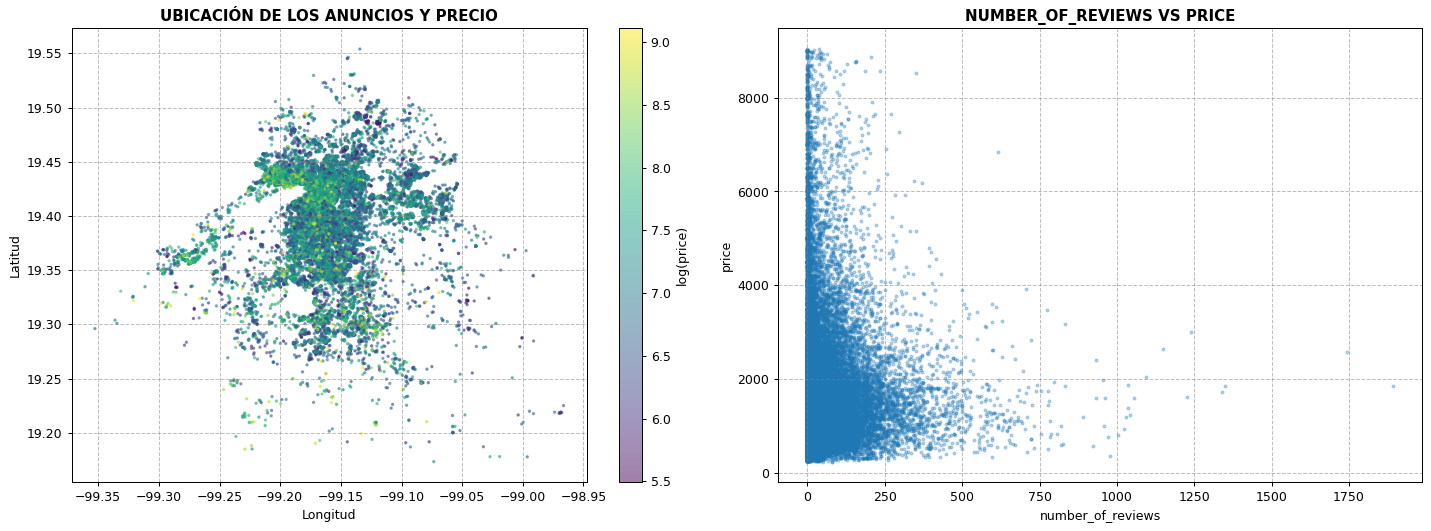
\includegraphics[width=\textwidth]{09_mapa_y_resenas_vs_precio.png}
  \caption{Distribución geográfica de los anuncios coloreada por $\ln(\texttt{price})$ (izquierda) y diagrama de dispersión de \texttt{number\_of\_reviews} frente a \texttt{price} (derecha).}
  \label{fig:mapa_resenas}
\end{figure}

El mapa confirma visualmente la correlación negativa con la longitud ($\rho = -0.226$): los anuncios se concentran densamente en el corredor centro-poniente (colonias Centro, Juárez, Roma, Condesa y Polanco), donde predominan los tonos verdes y amarillos asociados a los precios más altos, mientras que hacia el oriente y la periferia sur la densidad cae y predominan precios menores. Por su parte, la nube de dispersión entre \texttt{number\_of\_reviews} y \texttt{price} ($\rho = -0.018$) no muestra tendencia ascendente alguna; por el contrario, los alojamientos con mayor volumen histórico de reseñas ($>500$) operan casi exclusivamente en rangos de precio moderado (\$500--\$3,000 MXN), donde la rotación de huéspedes es mayor.

% ------------------------------------------------------------------------------
\section{Validación de la base de datos final}
\label{sec:validacion}

Para garantizar que la base de datos resultante es apta para el análisis estadístico formal, se ejecutó una validación integral en cuatro dimensiones: \textbf{completitud}, \textbf{consistencia}, \textbf{representatividad} y \textbf{relevancia}.

\subsection{Validación automatizada de completitud y consistencia}

Se programaron 13 aserciones booleanas sobre las bases finales (\texttt{df} y \texttt{df\_cod}); como muestra la Tabla~\ref{tab:validacion_reglas}, el \textbf{100\% de las verificaciones resultó satisfactorio}.

\begin{table}[htbp]
\centering
\caption{Resultados de las 13 pruebas automatizadas de validación de la base final.}
\label{tab:validacion_reglas}
\footnotesize
\renewcommand{\arraystretch}{1.12}
\begin{tabularx}{\textwidth}{c Y c}
\toprule
\rowcolor{TableHeader}
\textbf{\#} & \textbf{Regla de validación aplicada} & \textbf{Cumple} \\
\midrule
 1 & Sin nulos en variables de análisis (salvo \texttt{last\_review} estructural) & \cmark\ Sí \\
 2 & \texttt{last\_review} es nulo únicamente cuando \texttt{number\_of\_reviews == 0} & \cmark\ Sí \\
 3 & Base codificada (\texttt{listings\_final\_codificado.csv}) con cero valores nulos & \cmark\ Sí \\
 4 & Cero registros duplicados (ignorando \texttt{id}) & \cmark\ Sí \\
 5 & Identificador \texttt{id} estrictamente único & \cmark\ Sí \\
 6 & Todos los precios dentro de los límites de Tukey en logaritmo ($[\$241.82,\; \$9{,}058.85]$) & \cmark\ Sí \\
 7 & \texttt{minimum\_nights} acotada en el rango válido $[1,\; 365]$ & \cmark\ Sí \\
 8 & \texttt{availability\_365} dentro del rango válido $[0,\; 365]$ & \cmark\ Sí \\
 9 & Consistencia temporal: \texttt{number\_of\_reviews\_ltm <= number\_of\_reviews} & \cmark\ Sí \\
10 & Coordenadas geográficas contenidas en los límites de la CDMX & \cmark\ Sí \\
11 & Presencia íntegra de las 16 alcaldías de la Ciudad de México & \cmark\ Sí \\
12 & Presencia íntegra de los 4 tipos de alojamiento & \cmark\ Sí \\
13 & Base codificada 100\% numérica (37 columnas aptas para modelado) & \cmark\ Sí \\
\bottomrule
\end{tabularx}
\end{table}

\subsection{Validación de representatividad y estabilidad estadística}

Para comprobar que la eliminación del 9.47\% de los registros originales (inactivos, clonados y atípicos extremos) no introdujo sesgo en la estructura del mercado, se compararon las participaciones porcentuales originales y finales de cada clase de \texttt{room\_type} y \texttt{neighbourhood} (Tabla~\ref{tab:representatividad} y Figura~\ref{fig:representatividad}).

\begin{figure}[htbp]
  \centering
  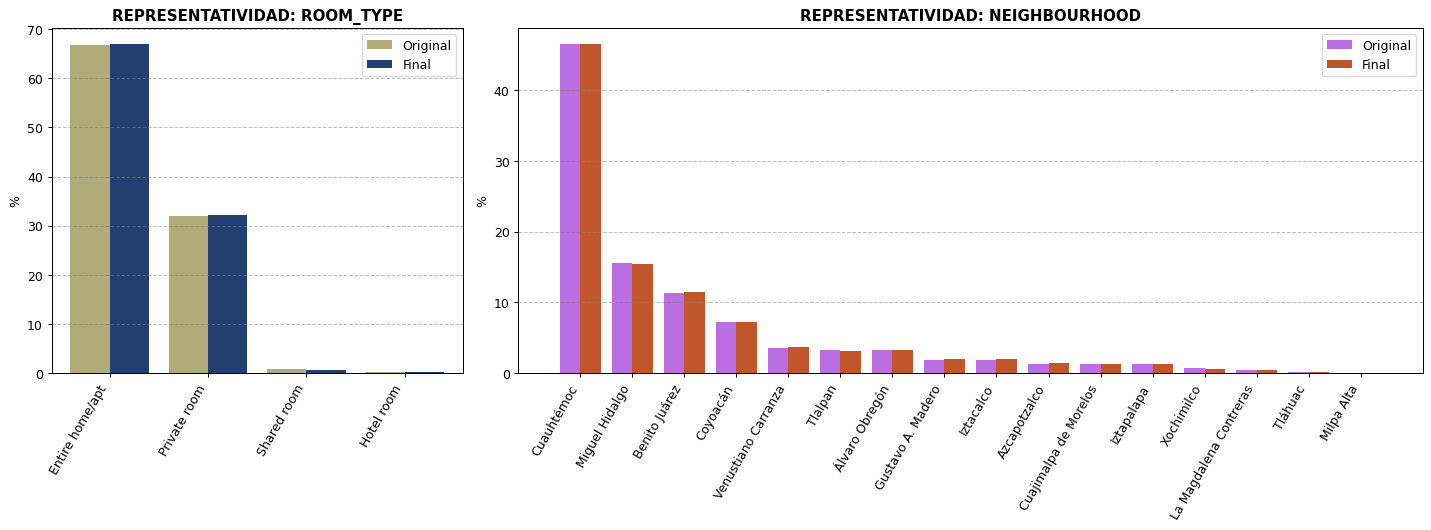
\includegraphics[width=\textwidth]{10_representatividad.png}
  \caption{Comparación de proporciones originales vs.\ finales por tipo de alojamiento y alcaldía.}
  \label{fig:representatividad}
\end{figure}

\begin{table}[htbp]
\centering
\caption{Evaluación de representatividad: proporciones originales ($n = 30{,}468$) vs.\ finales ($n = 27{,}583$).}
\label{tab:representatividad}
\scriptsize
\setlength{\tabcolsep}{3.5pt}
\renewcommand{\arraystretch}{1.1}
\begin{tabular}{l r r r | l r r r}
\toprule
\rowcolor{TableHeader}
\textbf{Categoría} & \textbf{\% Orig.} & \textbf{\% Final} & \textbf{Dif.\ (pp)} & \textbf{Categoría} & \textbf{\% Orig.} & \textbf{\% Final} & \textbf{Dif.\ (pp)} \\
\midrule
\multicolumn{4}{l|}{\textbf{\color{NavyPrimary}\texttt{room\_type}}} & Iztacalco              &  1.89 &  2.00 & $+0.11$ \\
Entire home/apt       & 66.78 & 66.94 & $+0.15$ & Iztapalapa             &  1.25 &  1.27 & $+0.02$ \\
Private room          & 32.07 & 32.11 & $+0.04$ & La Magdalena Contreras &  0.45 &  0.42 & $-0.03$ \\
Shared room           &  0.90 &  0.73 & $-0.17$ & Miguel Hidalgo         & 15.55 & 15.50 & $-0.06$ \\
Hotel room            &  0.25 &  0.22 & $-0.02$ & Milpa Alta             &  0.08 &  0.09 & $ 0.00$ \\
\cmidrule{1-4}
\multicolumn{4}{l|}{\textbf{\color{NavyPrimary}\texttt{neighbourhood}}} & Tlalpan                &  3.32 &  3.20 & $-0.12$ \\
Azcapotzalco          &  1.35 &  1.40 & $+0.05$ & Tláhuac                &  0.15 &  0.15 & $ 0.00$ \\
Benito Juárez         & 11.40 & 11.48 & $+0.08$ & Venustiano Carranza    &  3.62 &  3.64 & $+0.02$ \\
Coyoacán              &  7.25 &  7.25 & $ 0.00$ & Xochimilco             &  0.69 &  0.62 & $-0.07$ \\
Cuajimalpa de Morelos &  1.32 &  1.28 & $-0.04$ & Álvaro Obregón         &  3.28 &  3.26 & $-0.03$ \\
Cuauhtémoc            & 46.49 & 46.48 & $-0.02$ & \multicolumn{4}{r}{\textbf{Máxima dif.\ absoluta: 0.17 pp}} \\
Gustavo A.\ Madero    &  1.89 &  1.96 & $+0.07$ & \multicolumn{4}{r}{\textbf{Retención total: 90.53\%}} \\
\bottomrule
\end{tabular}
\end{table}

La diferencia máxima absoluta en cualquiera de las 20 categorías evaluadas es de apenas \textbf{0.17 puntos porcentuales} (\texttt{Shared room}: de 0.90\% a 0.73\%), y en las alcaldías principales la variación no supera los 0.12~pp. Adicionalmente, la Tabla~\ref{tab:comparativa_tres_etapas} compara los estadísticos de tendencia central y dispersión a lo largo de las tres etapas del proceso, demostrando que las medianas y los cuartiles se mantienen prácticamente estables mientras se elimina la distorsión artificial en la media y desviación estándar de \texttt{price}.

\begin{table}[htbp]
\centering
\caption{Evolución de los estadísticos descriptivos a través de las tres etapas de preparación.}
\label{tab:comparativa_tres_etapas}
\scriptsize
\renewcommand{\arraystretch}{1.13}
\begin{tabular}{l l r r r r r r}
\toprule
\rowcolor{TableHeader}
\textbf{Variable} & \textbf{Etapa} & \textbf{$N$} & \textbf{Media} & \textbf{DE} & \textbf{Q1} & \textbf{Mediana} & \textbf{Q3} \\
\midrule
\multirow{3}{*}{\texttt{price}}
  & Original            & 28,360 & 2,339.96 & 14,094.18 & 942.00 & 1,500.00 & 2,327.00 \\
  & Sin nulos de precio & 28,360 & 2,339.96 & 14,094.18 & 942.00 & 1,500.00 & 2,327.00 \\
  & \textbf{Final limpia} & \textbf{27,583} & \textbf{1,845.83} & \textbf{1,366.90} & \textbf{940.00} & \textbf{1,490.00} & \textbf{2,260.00} \\
\midrule
\multirow{3}{*}{\texttt{minimum\_nights}}
  & Original            & 30,467 & 2.92 & 16.03 & 1.00 & 1.00 & 2.00 \\
  & Sin nulos de precio & 28,359 & 2.33 &  9.92 & 1.00 & 1.00 & 2.00 \\
  & \textbf{Final limpia} & \textbf{27,583} & \textbf{2.25} & \textbf{8.68} & \textbf{1.00} & \textbf{1.00} & \textbf{2.00} \\
\midrule
\multirow{3}{*}{\texttt{number\_of\_reviews}}
  & Original            & 30,468 & 58.92 & 95.34 & 4.00 & 22.00 & 75.00 \\
  & Sin nulos de precio & 28,360 & 60.70 & 96.67 & 4.00 & 23.00 & 78.00 \\
  & \textbf{Final limpia} & \textbf{27,583} & \textbf{61.80} & \textbf{97.50} & \textbf{4.00} & \textbf{24.00} & \textbf{80.00} \\
\midrule
\multirow{3}{*}{\texttt{reviews\_per\_month}}
  & Original            & 26,385 & 2.01 & 2.28 & 0.57 & 1.47 & 2.79 \\
  & Sin nulos de precio & 24,778 & 2.07 & 2.30 & 0.63 & 1.56 & 2.86 \\
  & \textbf{Final limpia} & \textbf{27,583} & \textbf{1.84} & \textbf{2.27} & \textbf{0.34} & \textbf{1.28} & \textbf{2.66} \\
\midrule
\multirow{3}{*}{\texttt{availability\_365}}
  & Original            & 30,468 & 247.83 & 119.10 & 163.00 & 296.00 & 349.00 \\
  & Sin nulos de precio & 28,360 & 262.06 & 106.03 & 188.00 & 306.00 & 350.00 \\
  & \textbf{Final limpia} & \textbf{27,583} & \textbf{261.94} & \textbf{105.93} & \textbf{187.00} & \textbf{306.00} & \textbf{350.00} \\
\bottomrule
\end{tabular}
\end{table}

Finalmente, en cuanto a \textbf{relevancia}, todas las variables retenidas y generadas guardan relación directa con el objetivo estadístico del proyecto (ubicación espacial y administrativa, tipo de alojamiento, tarifa en escala original y logarítmica, condiciones de reserva y métricas de actividad/reseñas).

% ------------------------------------------------------------------------------
\section{Resultados, archivos generados y conclusiones}
\label{sec:conclusiones}

\subsection{Resumen cuantitativo del proceso y entregables}

La Tabla~\ref{tab:embudo_resultados} sintetiza el balance de registros depurados en cada etapa. Al concluir la metodología se exportaron dos archivos CSV verificados:

\begin{table}[htbp]
\centering
\caption{Balance de registros a lo largo del proceso de preparación de la base de datos.}
\label{tab:embudo_resultados}
\footnotesize
\renewcommand{\arraystretch}{1.15}
\begin{tabular}{l r r r}
\toprule
\rowcolor{TableHeader}
\textbf{Etapa del proceso} & \textbf{Eliminados} & \textbf{Restantes} & \textbf{\% del original} \\
\midrule
Base de datos original (\texttt{listings.csv}) & --- & 30,468 & 100.00\% \\
Eliminación de anuncios sin precio (inactivos) & 2,108 & 28,360 &  93.08\% \\
Eliminación de anuncios duplicados/clonados    &    79 & 28,281 &  92.82\% \\
Eliminación de precios atípicos (RIC en $\ln(\texttt{price})$) & 698 & \textbf{27,583} & \textbf{90.53\%} \\
\bottomrule
\end{tabular}
\end{table}

\begin{itemize}[leftmargin=1.5em]
  \item \textbf{\texttt{listings\_limpio.csv} ($27{,}583 \times 18$):} Base de datos limpia y legible, ideal para análisis exploratorio, tabulación cruzada, pruebas no paramétricas y visualizaciones.
  \item \textbf{\texttt{listings\_final\_codificado.csv} ($27{,}583 \times 37$):} Base de datos 100\% numérica, sin valores nulos y con codificación \textit{one-hot}, lista para regresión, análisis multivariado y algoritmos de modelado predictivo.
\end{itemize}

\subsection{Conclusiones}

\begin{enumerate}[leftmargin=1.5em]
  \item \textbf{Corrección efectiva de problemas estructurales:} La base original presentaba columnas 100\% vacías, nulos en la variable objetivo ligados a anuncios inactivos, nulos estructurales de reseñas, 79 registros clonados y valores extremos que inflaban la media y elevaban la asimetría del precio a 96.87. La metodología secuencial de siete etapas resolvió cada anomalía mediante criterios documentados y estadísticamente respaldados.
  \item \textbf{Calidad validada en cuatro dimensiones:} La base depurada conserva el \textbf{90.53\%} de los registros originales (27,583 anuncios) y satisface plenamente las propiedades de \textbf{completitud} (cero nulos no estructurales), \textbf{consistencia} (13 de 13 reglas aprobadas), \textbf{representatividad} (desviación máxima de 0.17~pp frente al mercado original) y \textbf{relevancia} analítica.
  \item \textbf{Evidencia exploratoria favorable a la hipótesis:} Los análisis gráficos y descriptivos indican que el \textbf{tipo de alojamiento} (alojamientos completos con mediana 2.12 veces mayor que habitaciones privadas) y la \textbf{ubicación geográfica} (corredor centro-poniente encabezado por Miguel Hidalgo, Cuajimalpa y Cuauhtémoc) son los factores más estrechamente asociados con el precio por noche, mientras que las variables de actividad exhiben correlaciones débiles ($|\rho| < 0.09$).
  \item \textbf{Recomendaciones para el análisis estadístico posterior (Capítulo~3):}
  \begin{itemize}[leftmargin=1.2em]
    \item Utilizar \texttt{log\_price} como variable respuesta en modelos paramétricos para satisfacer los supuestos de simetría y homocedasticidad.
    \item Emplear estadísticos robustos (mediana, RIC y pruebas no paramétricas) al comparar variables con colas largas.
    \item Evitar la inclusión simultánea de múltiples variables de reseñas (\texttt{number\_of\_reviews}, \texttt{reviews\_per\_month}, \texttt{number\_of\_reviews\_ltm} y \texttt{dias\_desde\_ultima\_resena}) para prevenir problemas de multicolinealidad ($|\rho|$ entre 0.57 y 0.88).
    \item En modelos de regresión con variables indicadoras (\textit{one-hot}), omitir una categoría de referencia por cada grupo (\texttt{room\_*}, \texttt{alc\_*}, \texttt{estancia\_*}) para evitar la trampa de las variables ficticias, e interpretar con cautela los coeficientes de categorías minoritarias (\texttt{Hotel room}, \texttt{Shared room}, Milpa Alta y Tláhuac).
  \end{itemize}
\end{enumerate}

% ==============================================================================
% REFERENCIAS BIBLIOGRÁFICAS
% ==============================================================================
\clearpage
\addcontentsline{toc}{chapter}{Referencias Bibliográficas}
\renewcommand{\bibname}{Referencias Bibliográficas}
\bibliographystyle{apalike}
\bibliography{referencias}

% ==============================================================================
% ANEXOS
% ==============================================================================
\appendix
\chapter{Estructura de la Base de Datos Codificada}
\label{anexo:columnas}

La Tabla~\ref{tab:anexo_columnas} enumera las \textbf{37 columnas numéricas} que integran el archivo final \texttt{listings\ub final\ub codificado.csv} ($27{,}583$ registros, $0$ valores nulos), agrupadas por su rol en el análisis estadístico y modelado.

\begin{table}[htbp]
\centering
\caption{Inventario completo de las 37 columnas de \texttt{listings\_final\_codificado.csv}.}
\label{tab:anexo_columnas}
\footnotesize
\renewcommand{\arraystretch}{1.2}
\begin{tabularx}{\textwidth}{>{\raggedright\arraybackslash}p{3.5cm} c Y}
\toprule
\rowcolor{TableHeader}
\textbf{Bloque} & \textbf{Cant.} & \textbf{Columnas incluidas} \\
\midrule
Llaves de identificación & 2 & \texttt{id}, \texttt{host\_id} (excluir como predictores en modelado). \\
\rowcolor{RowStripe}
Ubicación continua & 2 & \texttt{latitude}, \texttt{longitude}. \\
Variable objetivo & 2 & \texttt{price} (MXN), \texttt{log\_price} ($\ln(\texttt{price})$). \\
\rowcolor{RowStripe}
Condiciones y actividad & 8 & \texttt{minimum\_nights}, \texttt{number\_of\_reviews}, \texttt{reviews\_per\_month}, \texttt{calculated\_host\_listings\_count}, \texttt{availability\_365}, \texttt{number\_of\_reviews\_ltm}, \texttt{tiene\_resenas}, \texttt{dias\_desde\_ultima\_resena}. \\
Tipo de alojamiento (\textit{one-hot}) & 4 & \texttt{room\_Entire home/apt}, \texttt{room\_Hotel room}, \texttt{room\_Private room}, \texttt{room\_Shared room}. \\
\rowcolor{RowStripe}
Alcaldía (\textit{one-hot}) & 16 & \texttt{alc\_Azcapotzalco}, \texttt{alc\_Benito Juárez}, \texttt{alc\_Coyoacán}, \texttt{alc\_Cuajimalpa de Morelos}, \texttt{alc\_Cuauhtémoc}, \texttt{alc\_Gustavo A.\ Madero}, \texttt{alc\_Iztacalco}, \texttt{alc\_Iztapalapa}, \texttt{alc\_La Magdalena Contreras}, \texttt{alc\_Miguel Hidalgo}, \texttt{alc\_Milpa Alta}, \texttt{alc\_Tlalpan}, \texttt{alc\_Tláhuac}, \texttt{alc\_Venustiano Carranza}, \texttt{alc\_Xochimilco}, \texttt{alc\_Álvaro Obregón}. \\
Tipo de estancia (\textit{one-hot}) & 3 & \texttt{estancia\_Corta (1-7)}, \texttt{estancia\_Media (8-29)}, \texttt{estancia\_Larga (30+)}. \\
\bottomrule
\end{tabularx}
\end{table}

\end{document}
